% !TEX root = ../main.tex

\chapter{Experiments}
\label{chapter:Experiments}
The goal of our experimental evaluation is to analyze the performance of our algorithm in the key aspects of 
\ac{il}, \ac{rl} with expert demonstrations and \ac{rl} without expert demonstrations. 

We will compare pure \ac{il} of our algorithm in the deterministic \ac{sopomdp} of the 
natural language conditioned robot manipulation task benchmark as described in appendix \ref{LCILRM} using the provided baseline.

Then we will use environments from the Meta-World benchmark as described in appendix \ref{chapter:MetaWorld} for both \ac{sopomdp}s and \ac{mdp}s.

We first investigate the effect of different search paradigms in inference time for the \ac{avc} algorithm, as described in section Inference Time Search \ref{sec:inf_time_search}.

To compare our results, we use \ac{ppo} and \ac{tqc} for the \ac{rl} algorithms, as they are state-of-the-art with respect to stability and 
exploration respectively. For the base implementations, we use "Stable Baselines3" \cite{stable-baselines3}, which is a common choice, as it provides well-implemented algorithms with tested
performance and fine-tuned hyperparameters for a wide range of environments. This includes our chosen environments, but with dense rewards and continued observations,
thus some hyperparameter tuning is necessary.

In settings where \ac{il} is key, we use \ac{gail} to provide dense rewards for the reinforcement learners to make best use of the provided expert demonstrations.

In settings with focus on \ac{rl} we use the provided sparse reward from the environment. In some settings, we provide one 
expert demonstration to guide initial exploration. Here, we use behavioral cloning as pretraining for the baselines and the sparse rewards from the environment during the reinforcement phase. 
We will investigate the effect of these choices on the performance of the baseline algorithms.

In the deterministic \ac{sopomdp} setting, we will use the strong inductive bias described in the "Curse Of Dimensionality" 
Section \ref{COD_AC} for \ac{tqc} and \ac{ppo} to encode the current belief state of the environment.

Specifically, we encode the current history by appending a positional encoding to the initial observation. The upside is that we give 
the baseline algorithms a way to make use of the determinacy of the environment by reducing the preimage of the algorithms compared to 
frame stacking. The downside is, that the algorithms have no information about previously taken actions. Therefor we use the 
algorithms in deterministic mode in test time. We derived, why this is sufficient in our discussion of the strong inductive bias in 
Section \ref{COD_AC}.

We also include a standard algorithm for \ac{pomdp}s, namely RPPO. It does not make use of the strong inductive bias but uses a GRU 
to encode the belief state, giving it access to previous actions and the initial observation.


In summary, we will first investigate \ac{avc} on pure \ac{il}. Then we analyze different inference time search 
paradigms for \ac{rl}. We will compare \ac{avc} with \ac{rl} in the deterministic \ac{sopomdp} setting to our chosen baselines and finally we analyze 
\ac{rl} of \ac{coavc} in the \ac{mdp} setting.


\section{Imitation Learning}
\label{sec:exp_imi_lr}
In this section, we present our findings on the natural language conditioned robot manipulation task benchmark as described in appendix \ref{LCILRM} that was proposed by 
Simon Stepputtis \etAl \cite{stepputtis2020languageconditioned}. The benchmark consists of a 7 dof simulated robot arm with a 
tabletop setup using CoppeliaSim. The task is to pick 
up the correct cup and pour the content into the correct bowl, using natural language description of the cup and bowl and an RGB 
picture of the scene.

In this experiment, only the first observation consisting of the RGB values from the picture of the 
scene and the task description is visible for the actor. The method \ac{lcil} 
proposed by the authors uses a recurrent policy. As we have motivated in Section \ref{COD_AC}, we expect our method to perform better than autoregressive or recurrent 
models because we use the knowledge that we are not getting additional information from the environment during the unroll of the trajectory. 
To test this, we have used the dataset of 40,000 expert demonstrations provided with the benchmark to train our model using only \ac{il}.
\begin{table}
  \centering
  \begin{tabular}{|c|c|c|}
      \cline{2-3}
      \multicolumn{1}{c|}{} & \textbf{Active Critic} & \textbf{LCIL} \\ \hline
      \textbf{Pick} & 100 \% & 98 \% \\ \hline
      \textbf{Pour} & 99 \% & 95 \% \\ \hline
      \textbf{Combined} & 98 \% & 92 \% \\ \hline
  \end{tabular}
  \caption{Success rates of the 100 pick, pour and combined tasks. The left column depicts the results from the \ac{avc} algorithm (ours) in 
  imitation mode. Right is the result of the \ac{lcil} architecture.}
  \label{tab:lcil}
\end{table}

The results are depicted in table \ref{tab:lcil}. On the 100 test environments that were provided, we decreased the overall error rate by 75$ \% $. 
\begin{figure}
    \captionsetup[subfigure]{justification=Centering, labelformat=empty}
    \begin{subfigure}[t]{0.18\textwidth}
        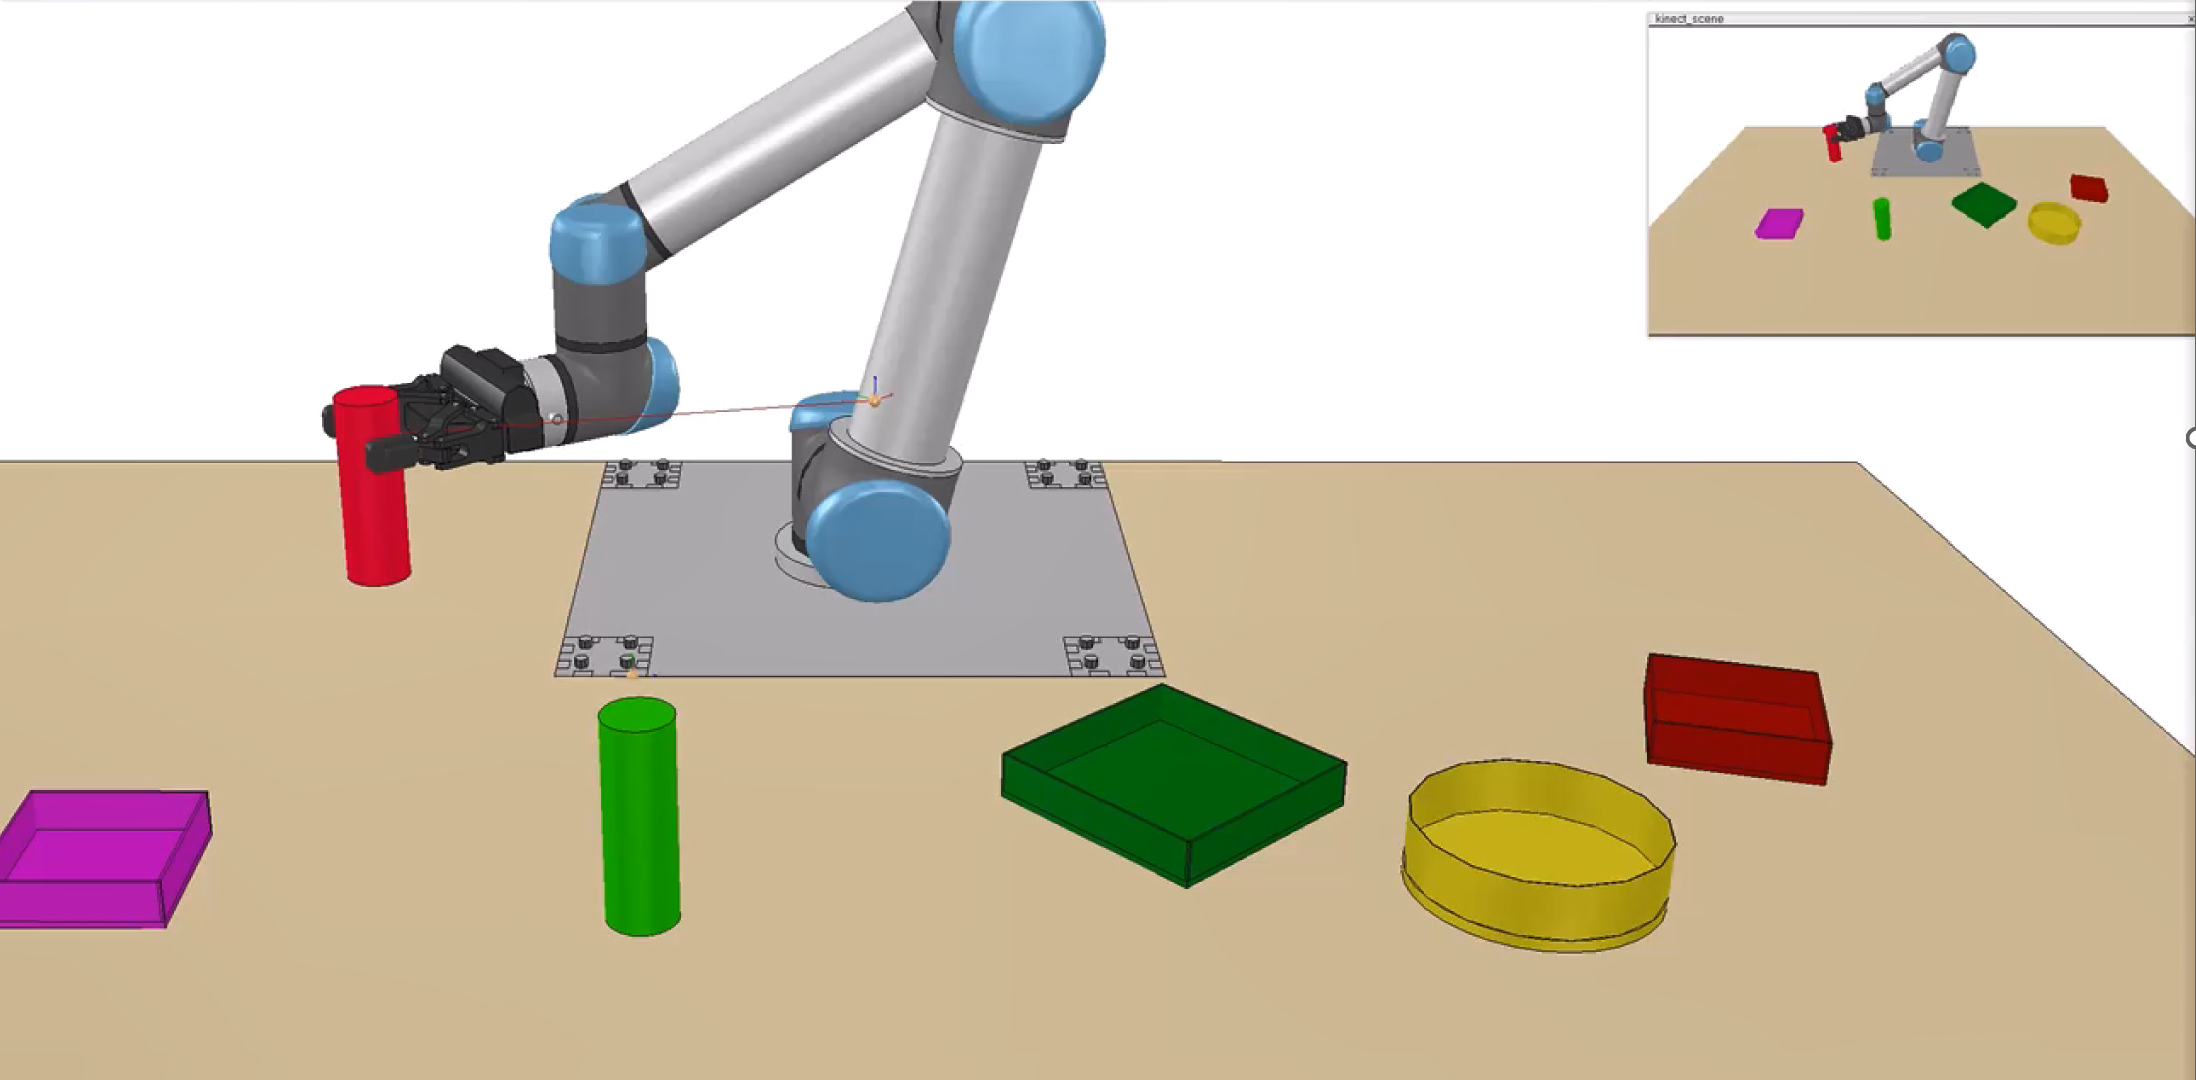
\includegraphics[width=\textwidth]{images/Language_Conditioned_Exp/theirs_1.png}
        \caption{Time step 60.}
    \end{subfigure}
    \begin{subfigure}[t]{0.18\textwidth}
        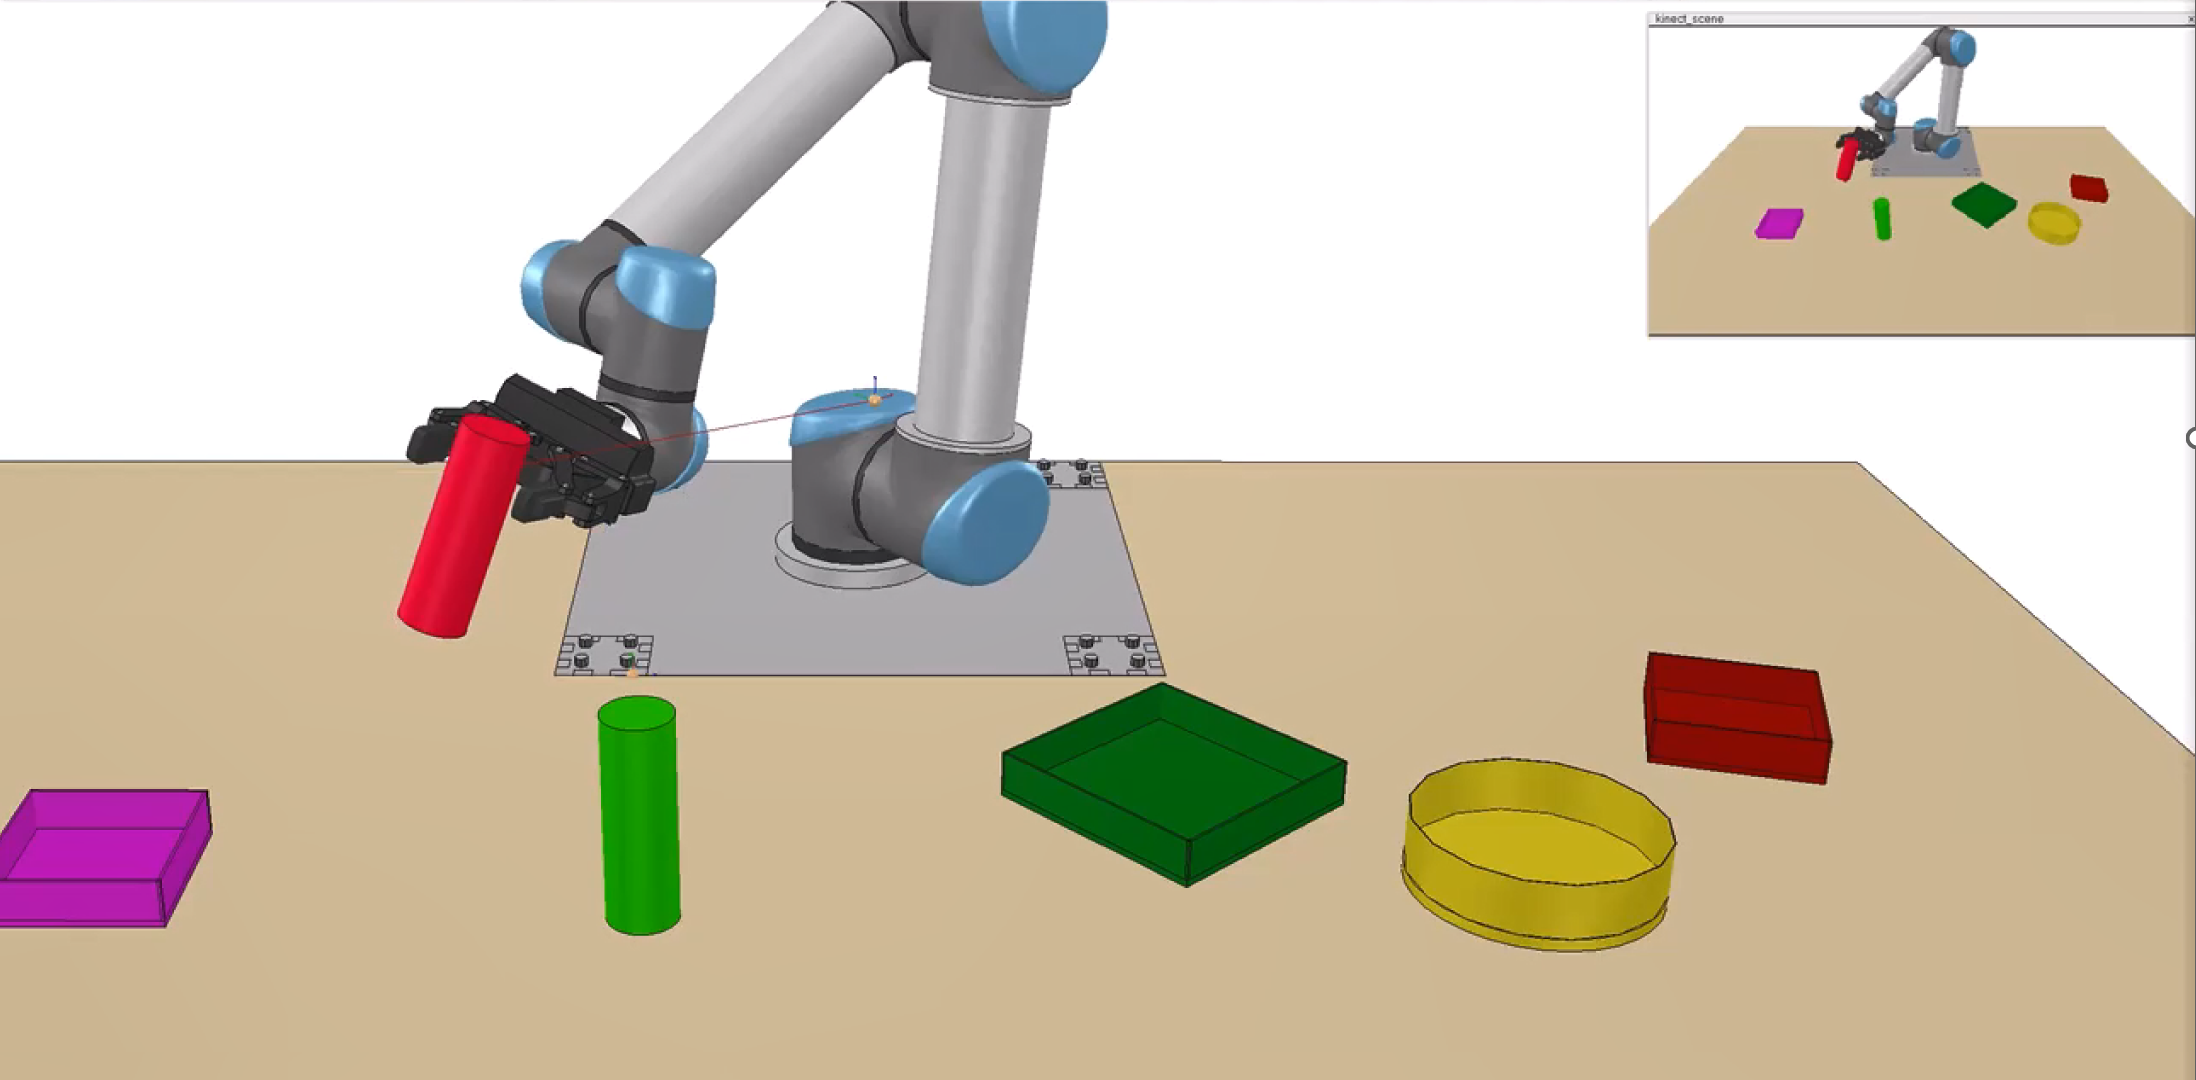
\includegraphics[width=\linewidth]{images/Language_Conditioned_Exp/theirs_2.png}
        \caption{Time step 120.}
    \end{subfigure}
    \begin{subfigure}[t]{0.18\textwidth}
        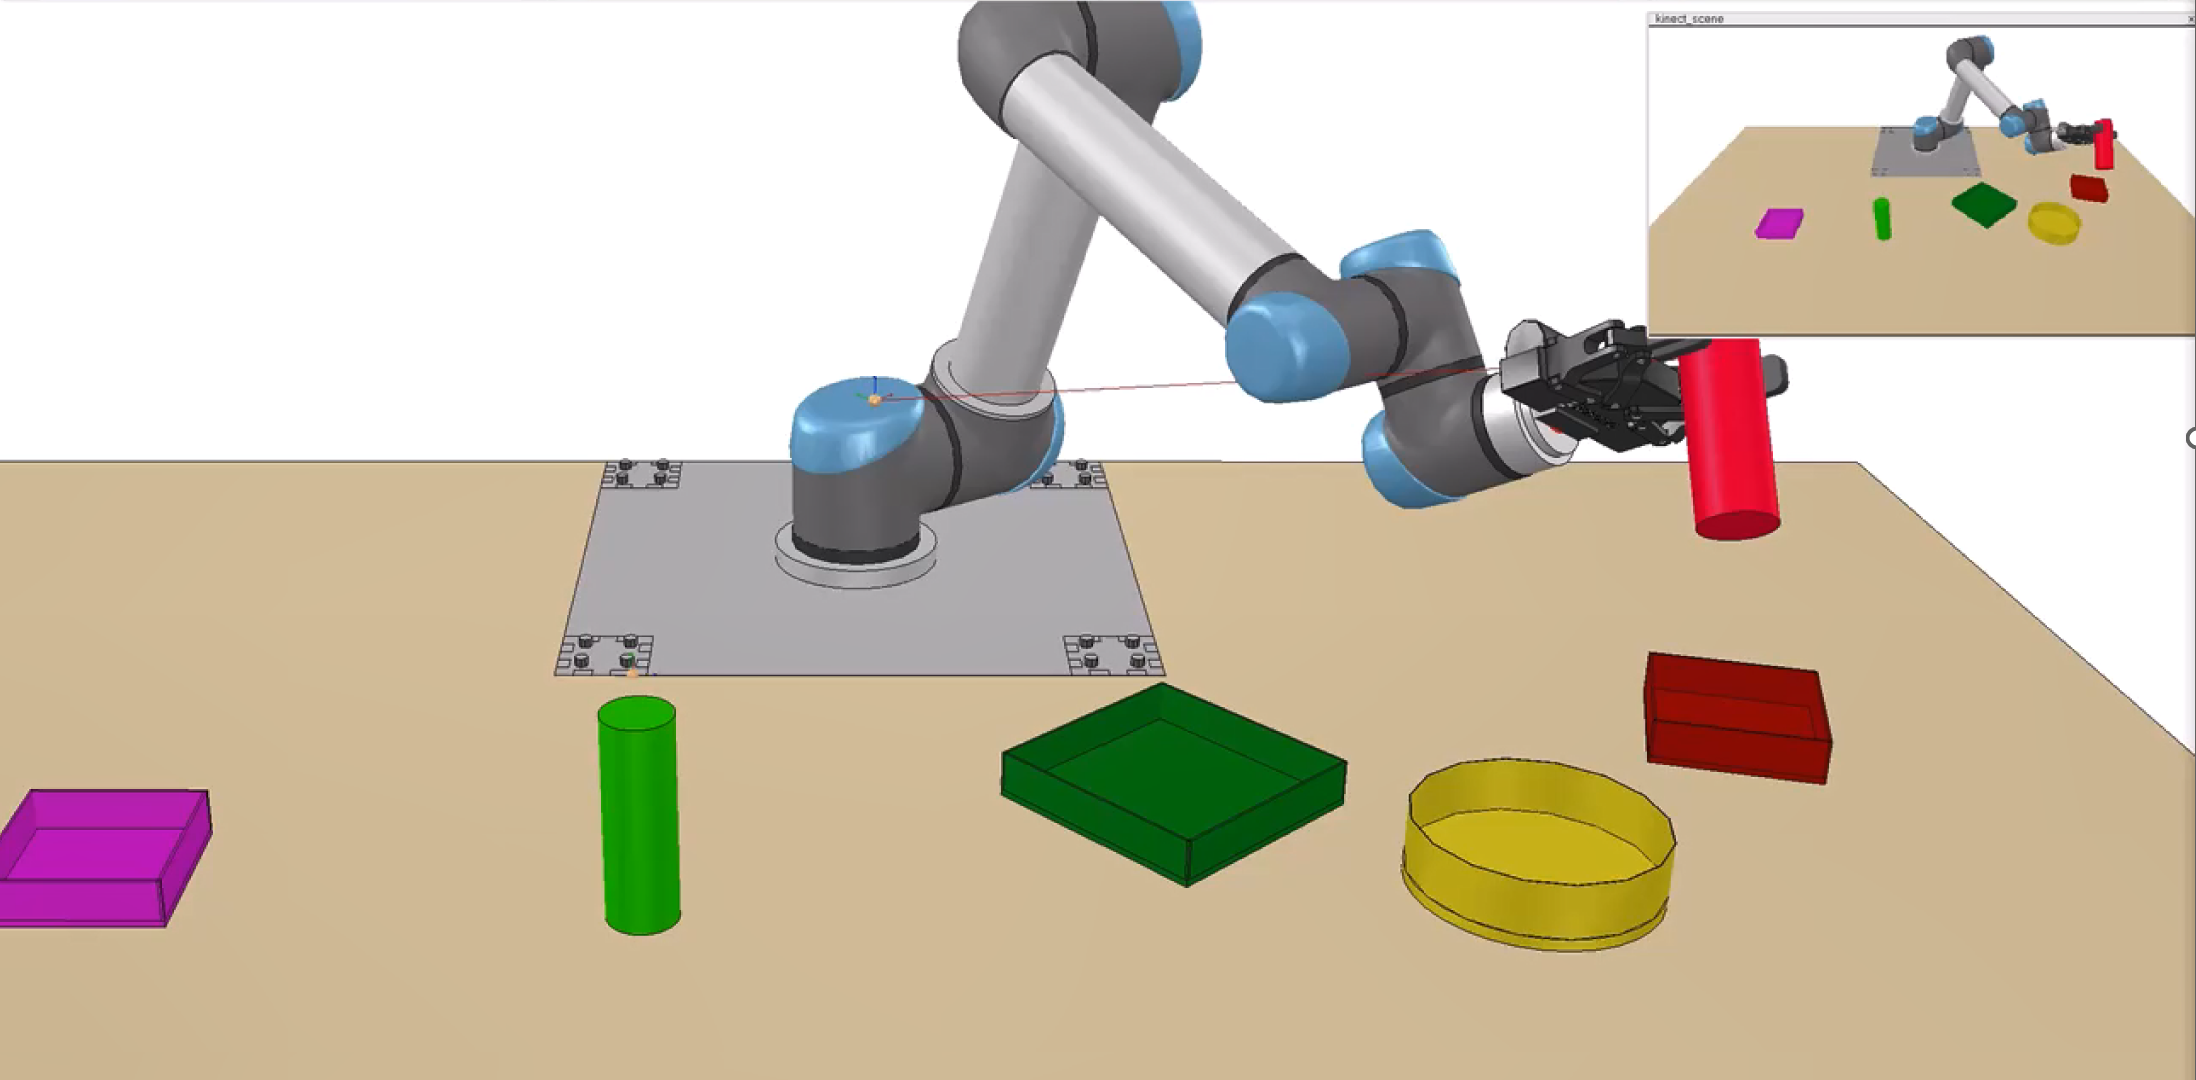
\includegraphics[width=\linewidth]{images/Language_Conditioned_Exp/theirs_3.png}
        \caption{Time step 180.}
    \end{subfigure}
    \begin{subfigure}[t]{0.18\textwidth}
        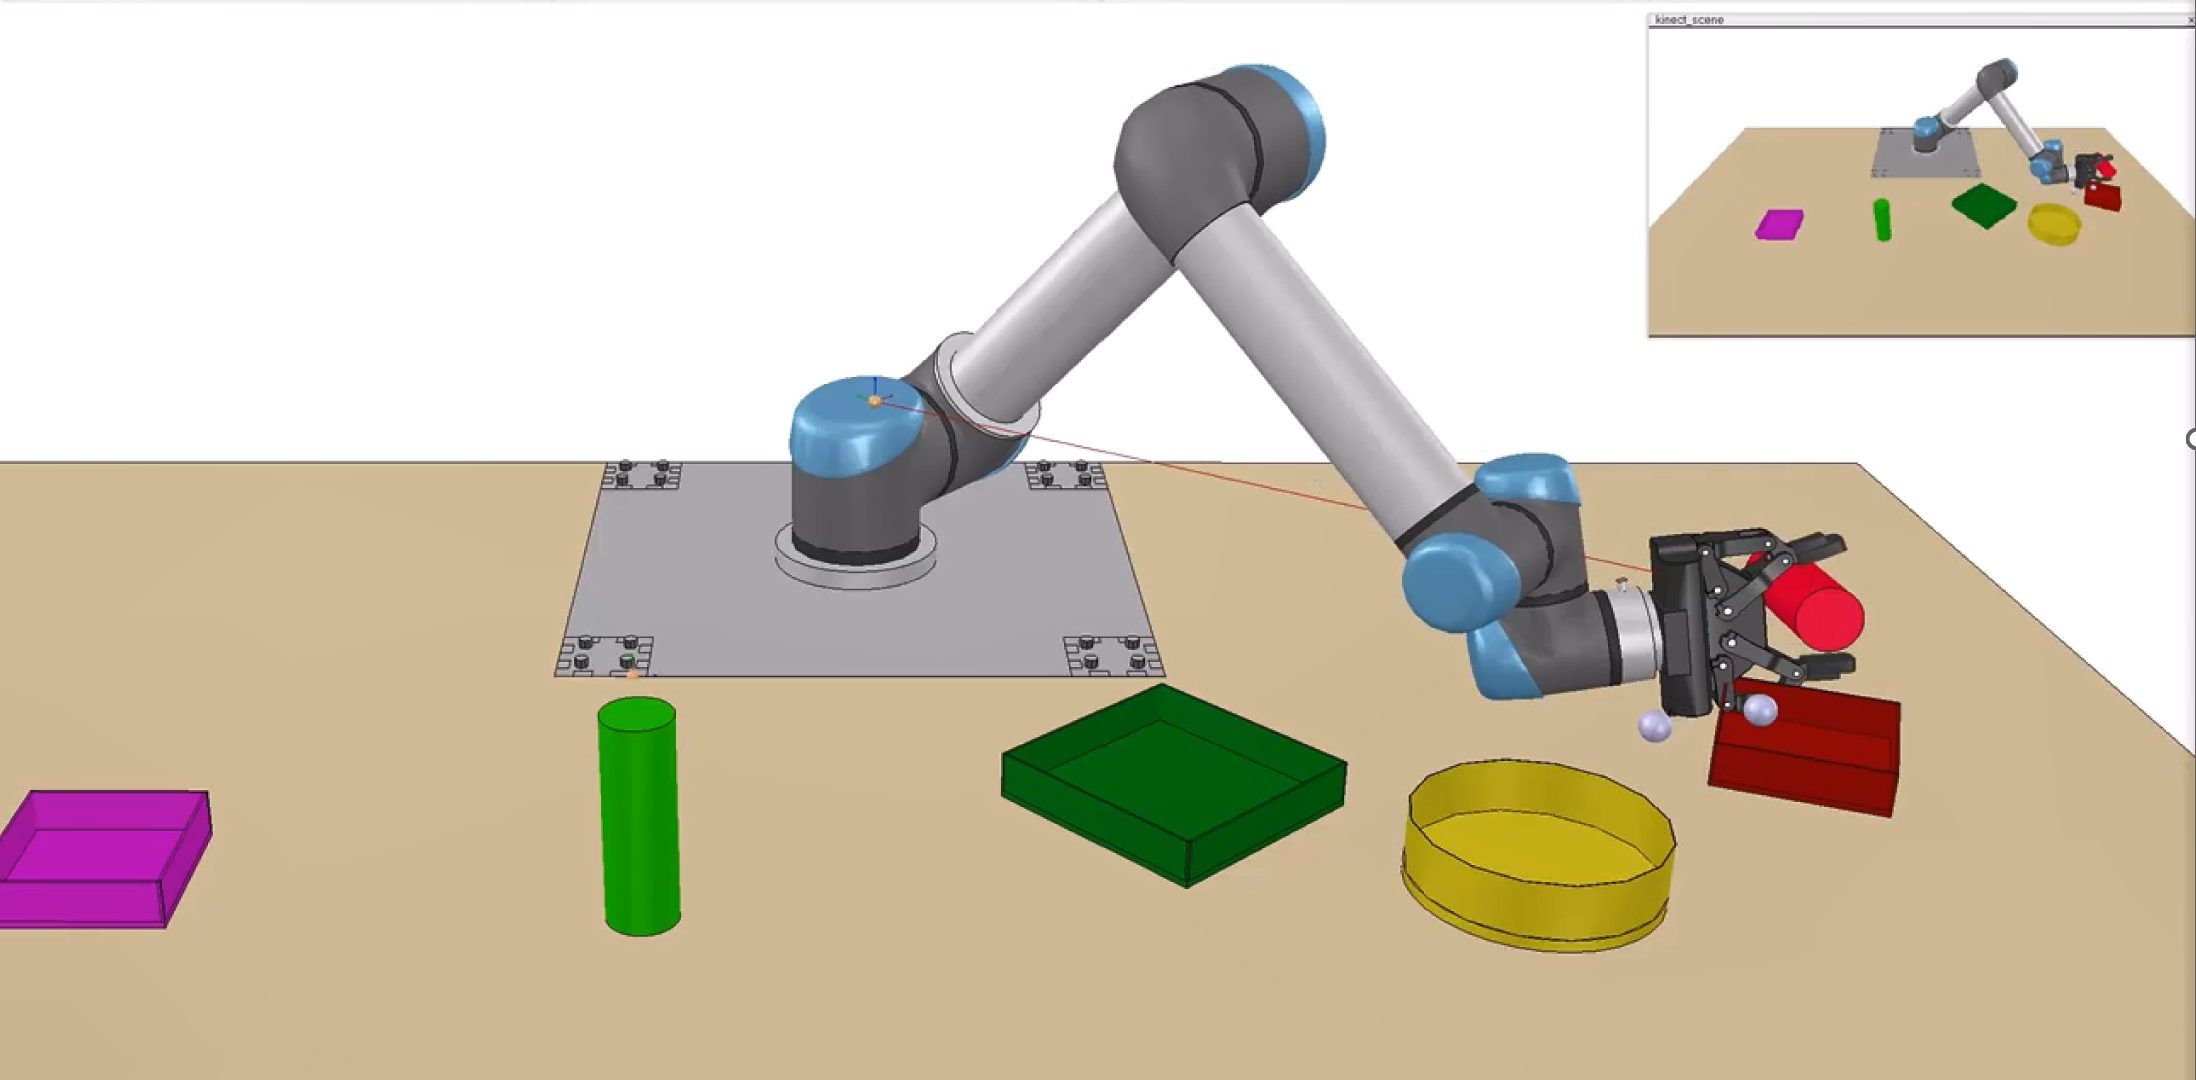
\includegraphics[width=\linewidth]{images/Language_Conditioned_Exp/theirs_4.png}
        \caption{Time step 240.}
    \end{subfigure}
    \begin{subfigure}[t]{0.18\textwidth}
        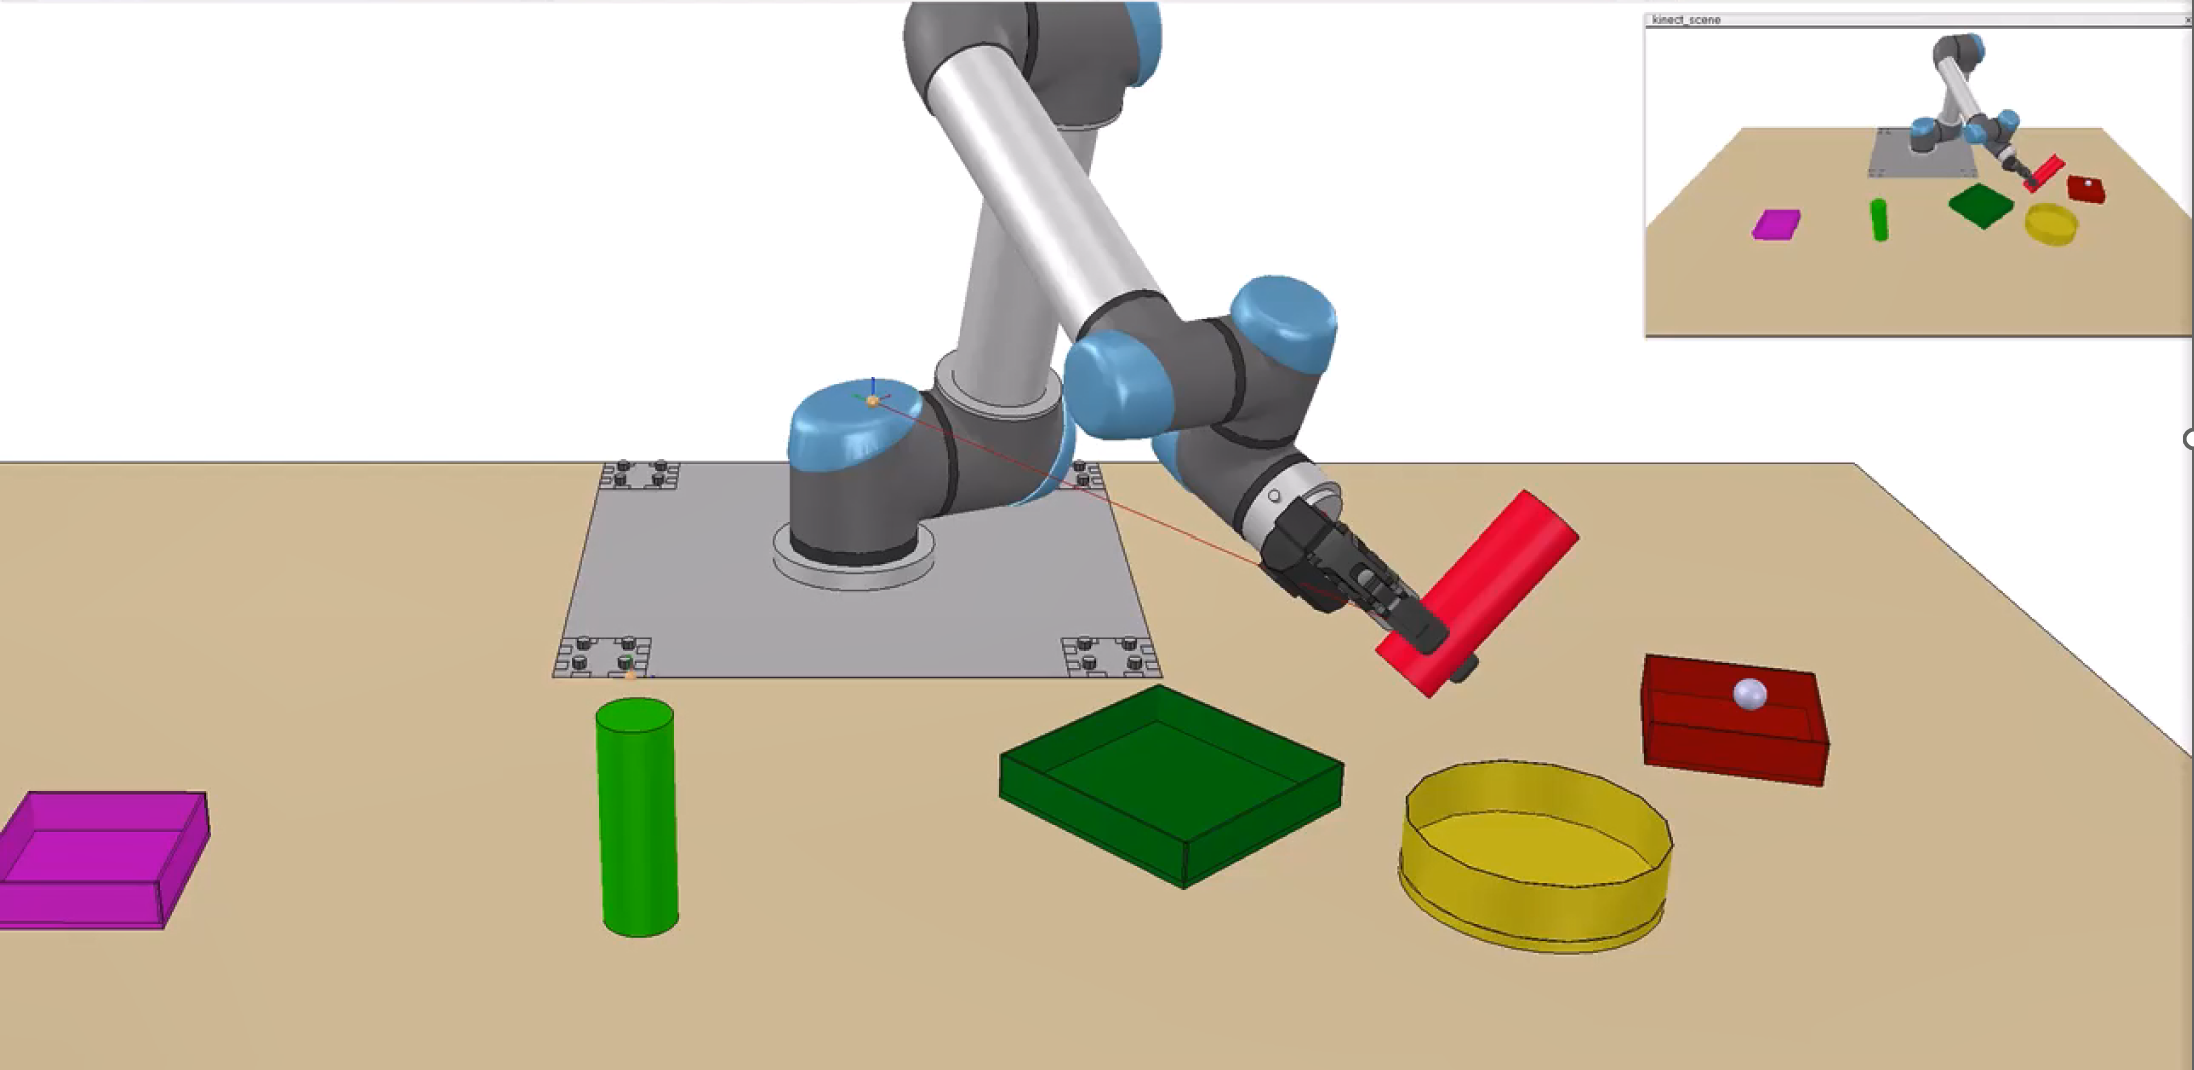
\includegraphics[width=\linewidth]{images/Language_Conditioned_Exp/theirs_5.png}
        \caption{Time step 300.}
    \end{subfigure}

    \bigskip % more vertical separation
    \begin{subfigure}[t]{0.18\textwidth}
        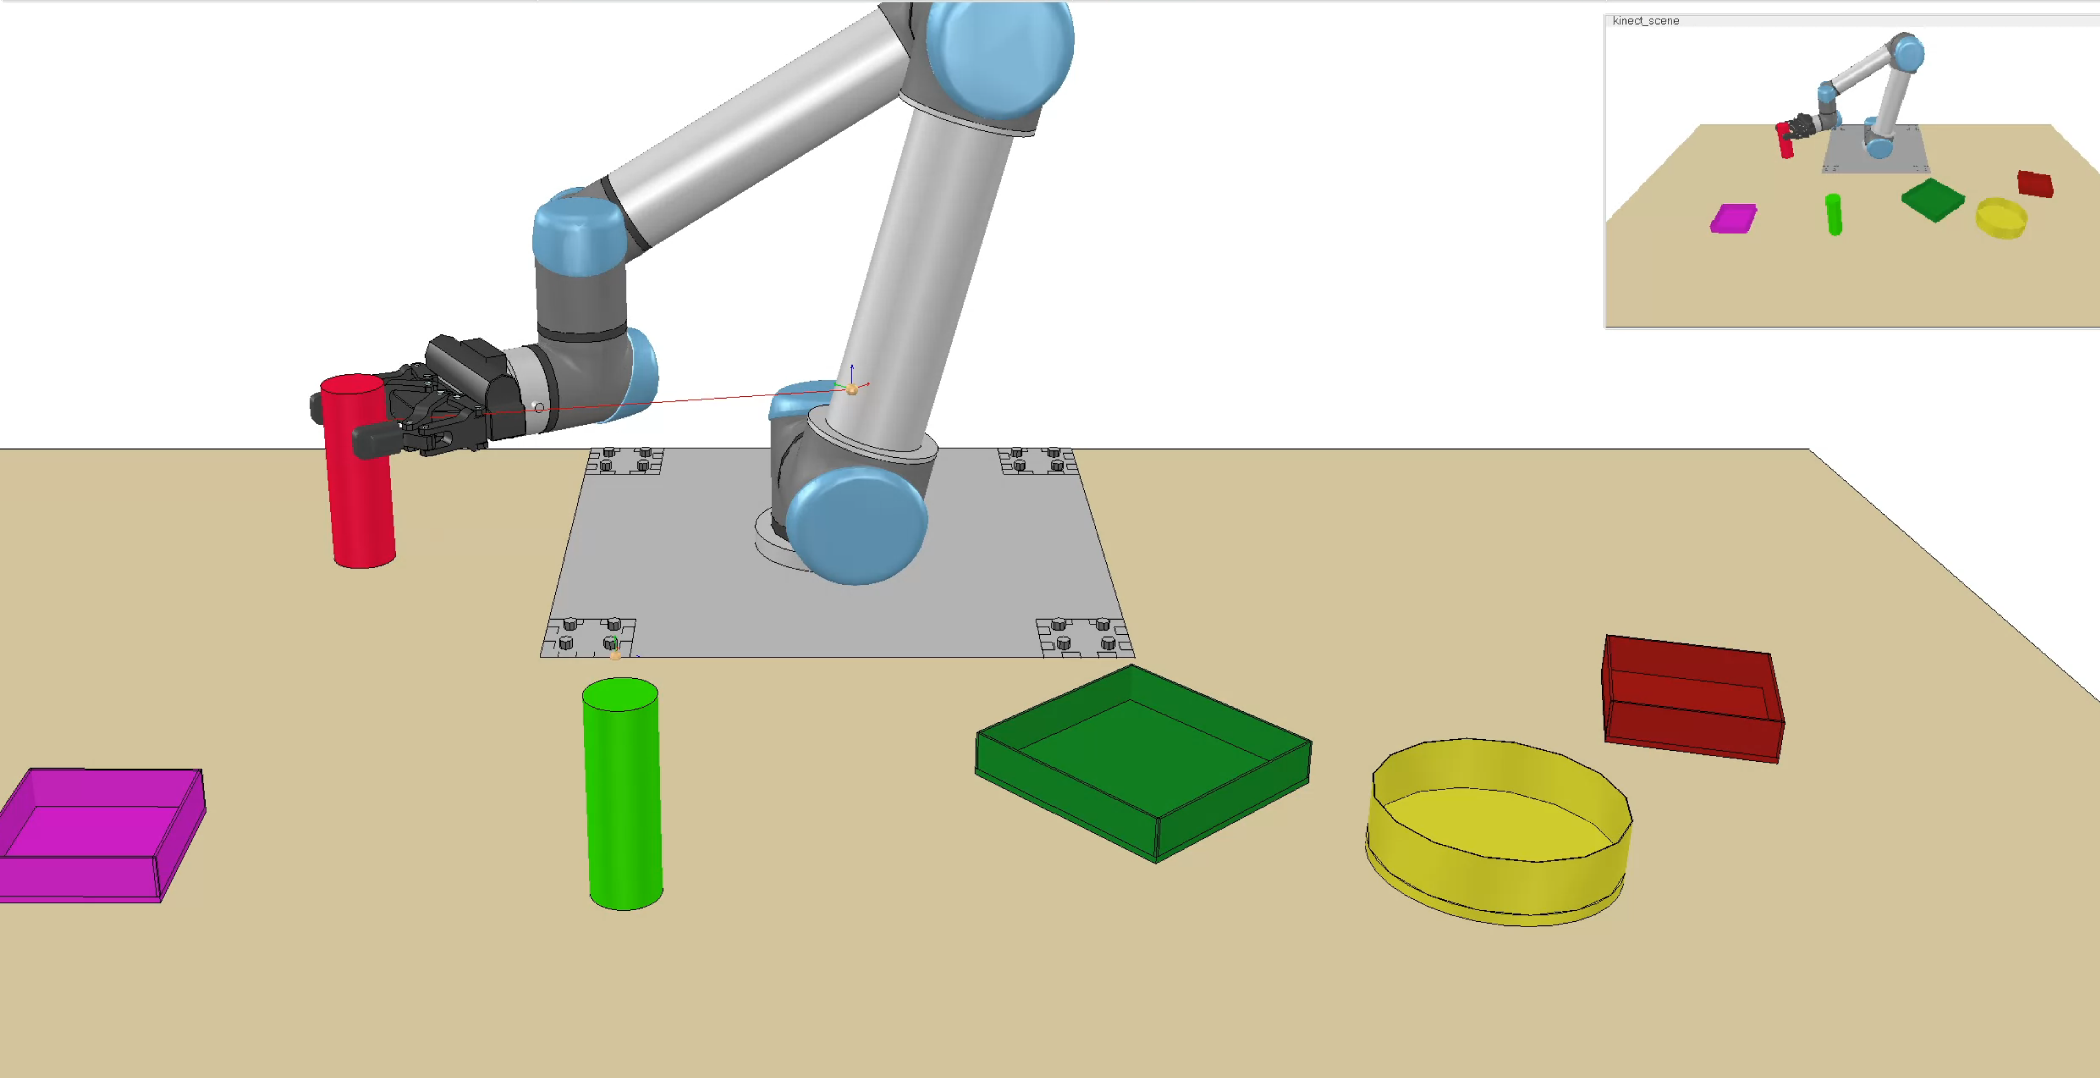
\includegraphics[width=\linewidth]{images/Language_Conditioned_Exp/mine_1.png}
        \caption{Time step 60.}
    \end{subfigure}
    \begin{subfigure}[t]{0.18\textwidth}
        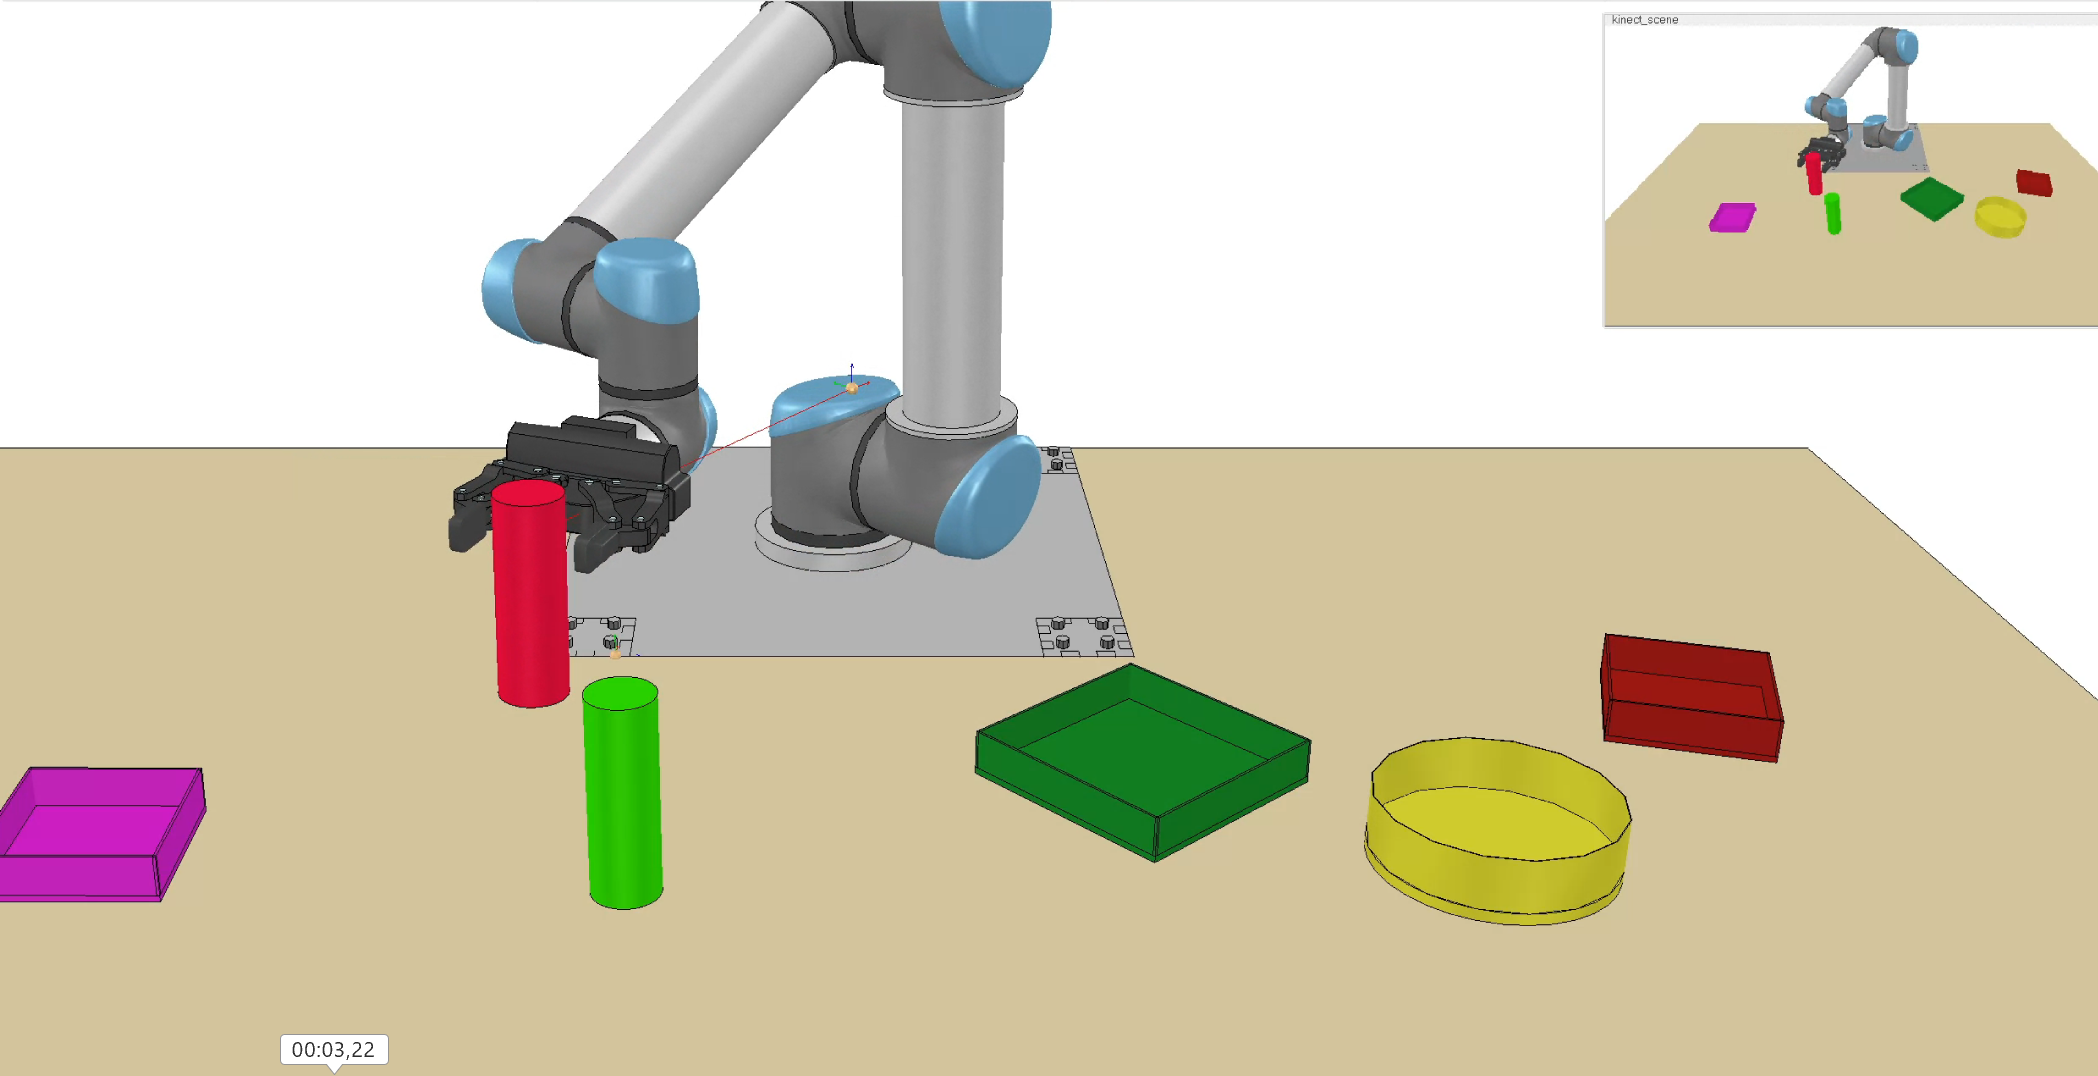
\includegraphics[width=\linewidth]{images/Language_Conditioned_Exp/mine_2.png}
        \caption{Time step 120.}
    \end{subfigure}
    \begin{subfigure}[t]{0.18\textwidth}
        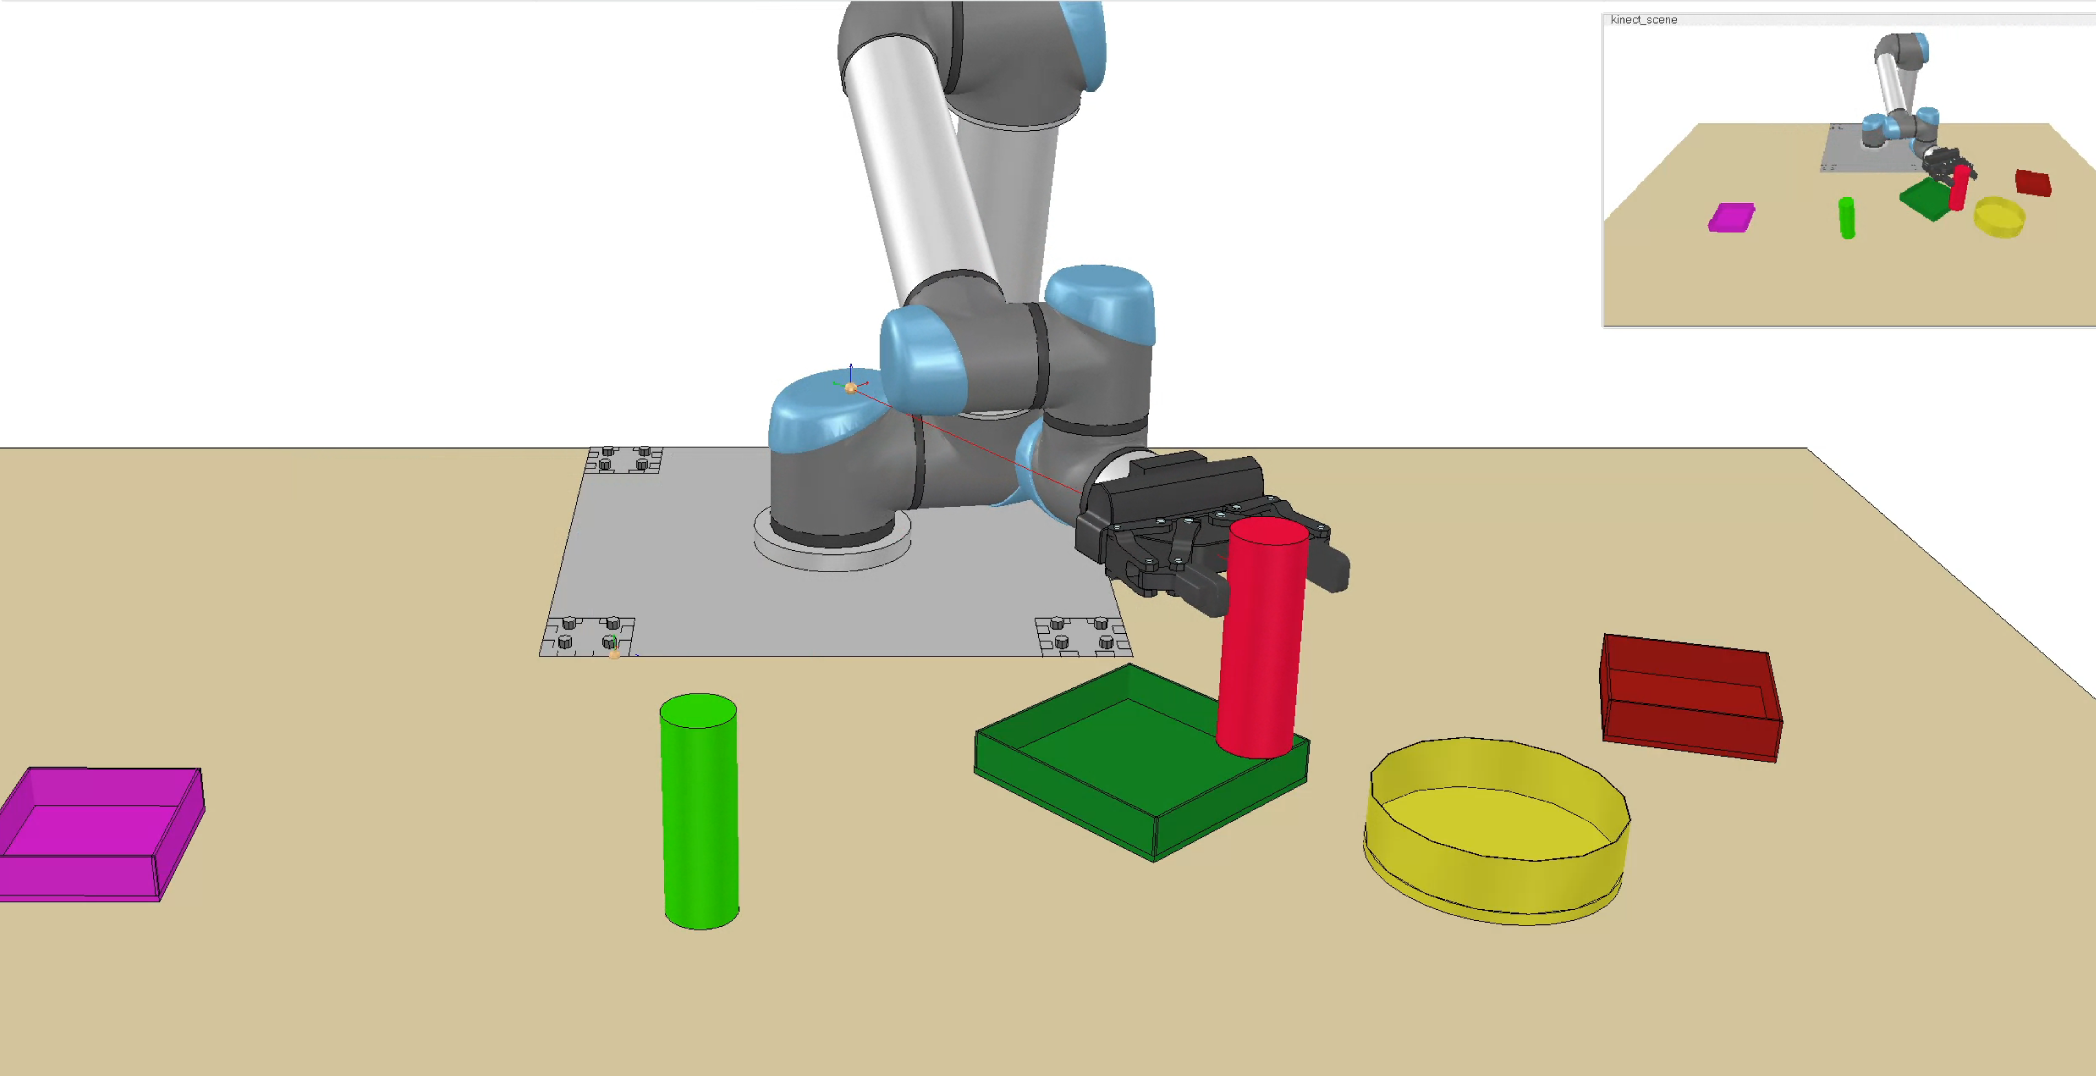
\includegraphics[width=\linewidth]{images/Language_Conditioned_Exp/mine_3.png}
        \caption{Time step 180.}
    \end{subfigure}
    \begin{subfigure}[t]{0.18\textwidth}
        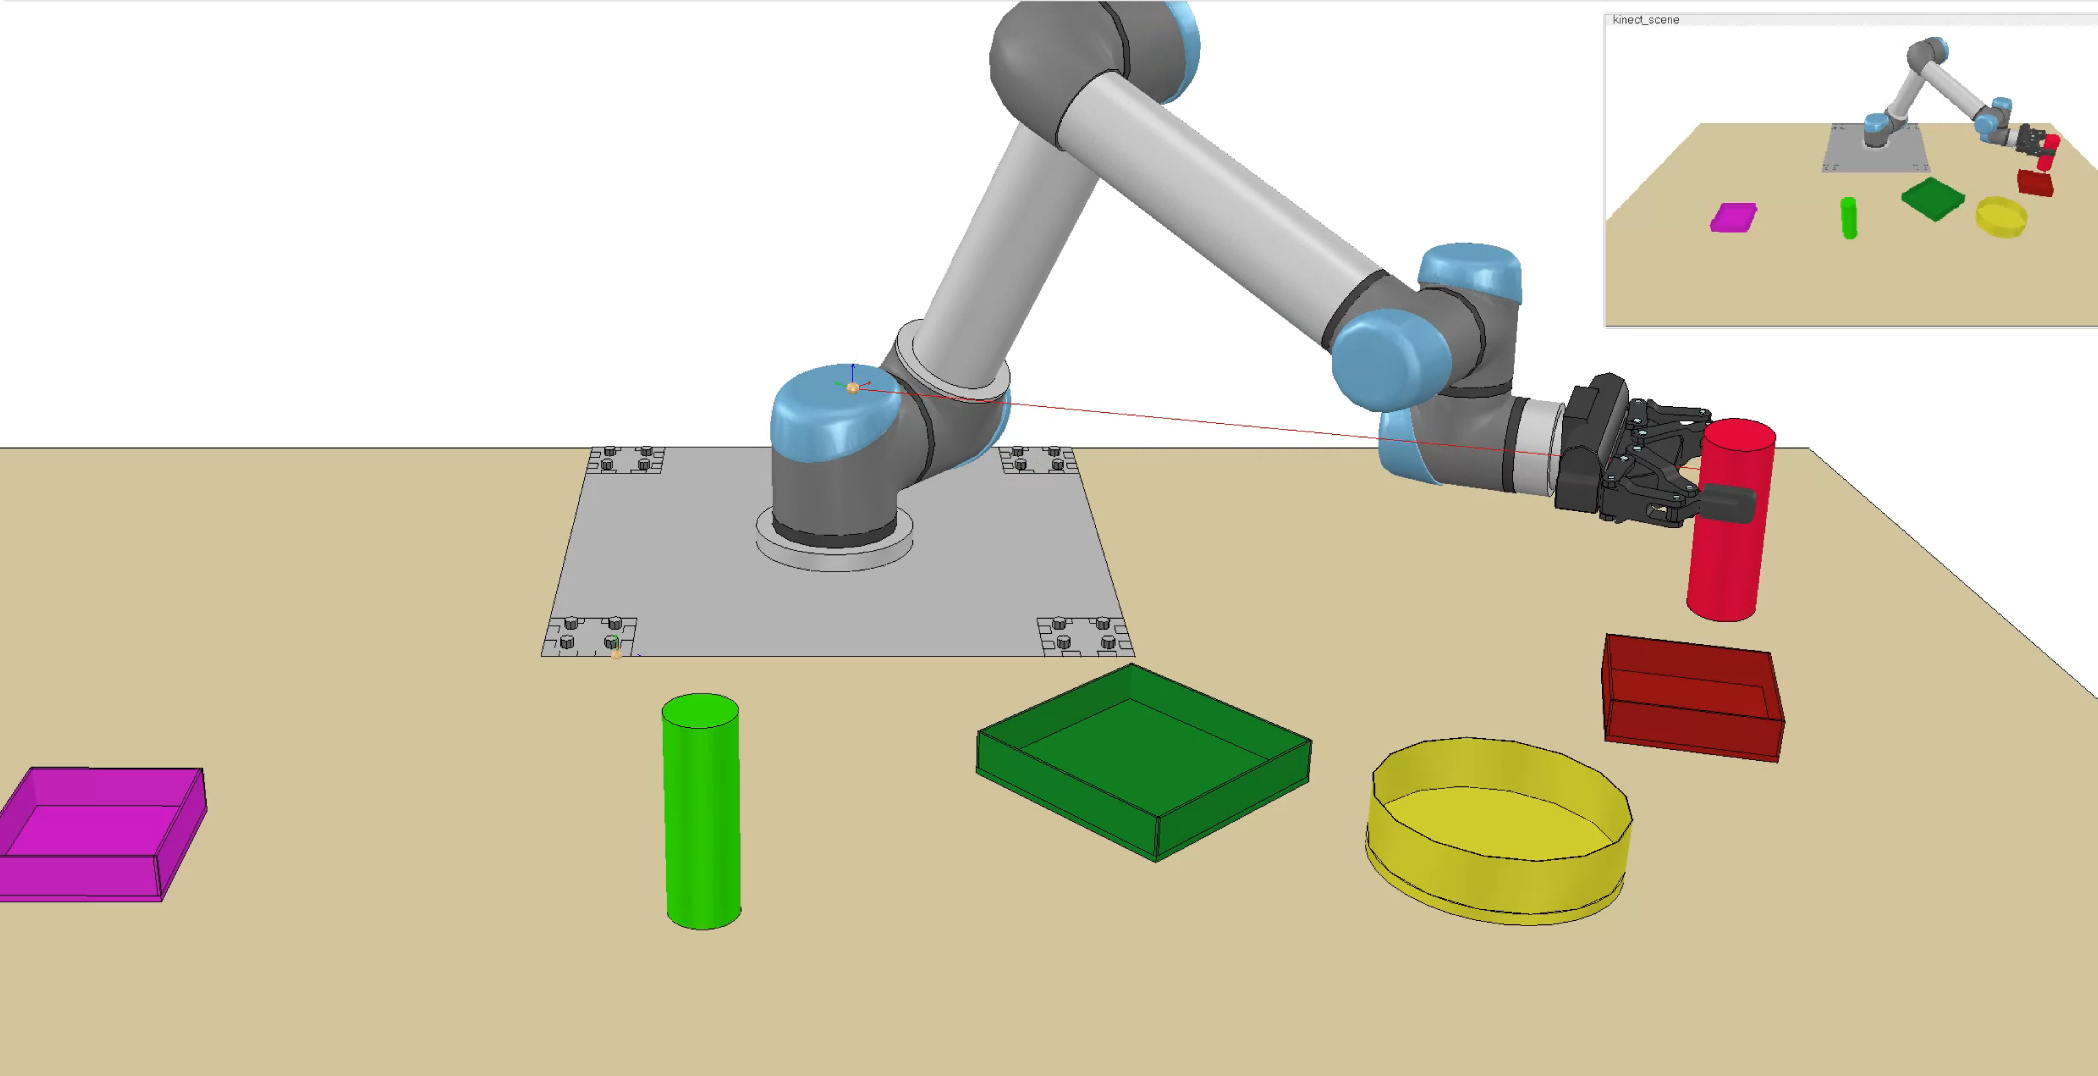
\includegraphics[width=\linewidth]{images/Language_Conditioned_Exp/mine_4.png}
        \caption{Time step 240.}
    \end{subfigure}
    \begin{subfigure}[t]{0.18\textwidth}
        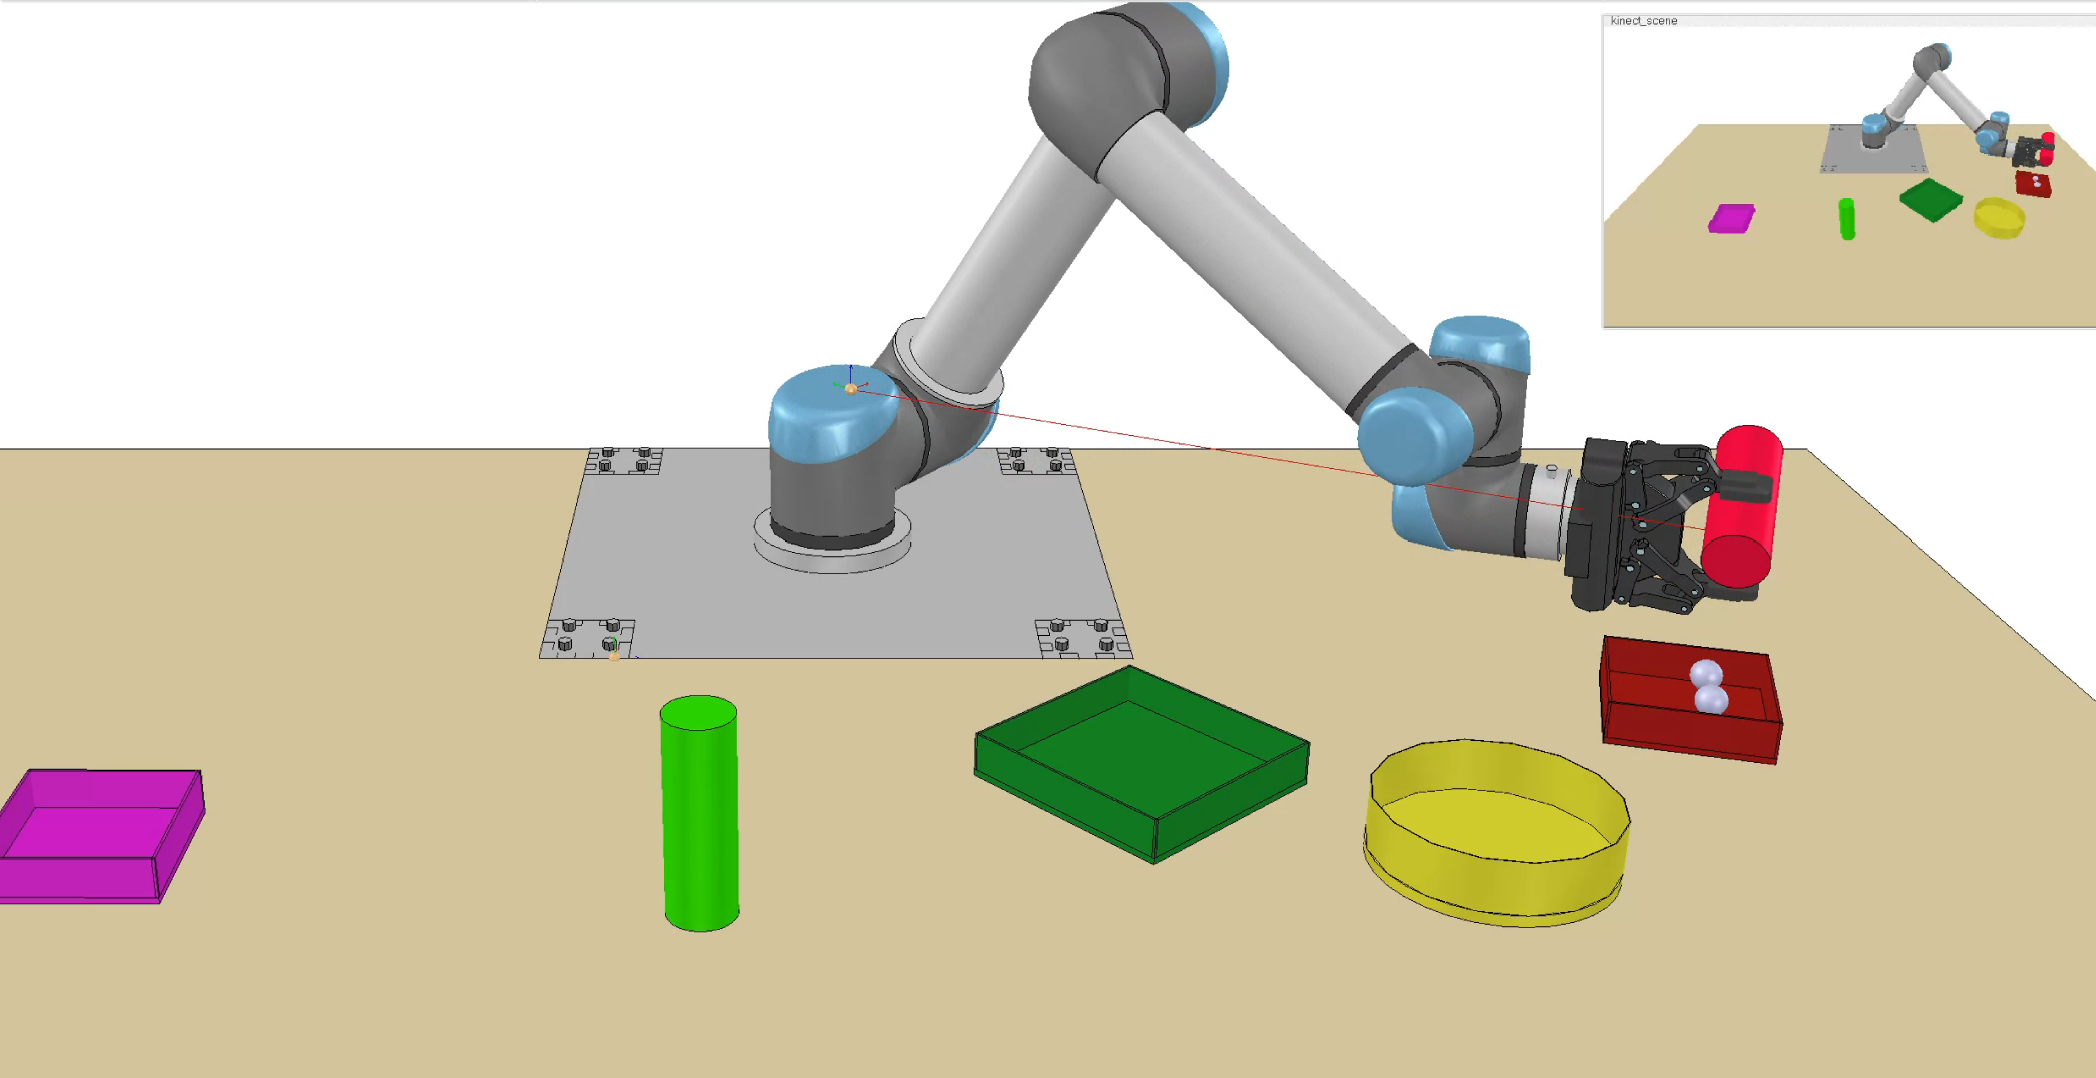
\includegraphics[width=\linewidth]{images/Language_Conditioned_Exp/mine_5.png}
        \caption{Time step 300.}
    \end{subfigure}
    \caption{Comparison of a pour task. The policy learned by the \ac{lcil} algorithm (top row) spills the content over the table and moves unpredictable. The task is considered a failure 
    by the benchmark, as most drops did not land in the goal bowl. \ac{avc} (bottom row) performs the task as intended with no unexpected movement.}
    \label{fig: AVC vs. Rec}
\end{figure}
In Figure \ref{fig: AVC vs. Rec}, we have depicted a case in the test dataset that our policy solved and compared it to the performance 
of the recurrent algorithm, which failed at the task. 

While our approach hit the target precisely, the recurrent model was widely off. We assume that this is caused by the fact that during inference 
time, the
\ac{iid} assumption of the input data to the policy is broken. Intuitively, the recurrent policy
is in a state that it has not seen before and acts slightly differently to the expert. After some steps, the policy now sees 
inputs that are vastly
different from the training distribution, thus it starts to act unpredictably. As argued in Section \ref{COD_AC}, this is an advantage of our 
policy as in our inference method the \ac{iid} assumption holds.

\section{Reinforcement Learning from Sparse Rewards in Single Observation Environments}
In this section, we will explore the performance of the \ac{avc} algorithm given a single observation per trajectory, one sparse reward, and some expert demonstrations.
We motivated the practical relevance in the introduction. An additional advantage for testing the effectiveness of the search paradigm is that planning is most efficient in
single observation settings.
We discussed this in Section \ref{sec:AC_Critic}, where we state that while predicting the \ac{mdp} has a quadratic error bound, we don't get any updated information
during the trajectory, and thus no better estimate is possible then the prediction at time step $1$. 

We chose environments from the Meta-World benchmark as described in appendix \ref{chapter:MetaWorld}. 
Specifically we chose five environments from the ML10 suite, namely Pick and Place, Push, Reach, Window Open and Drawer Close, which represent a variety
of difficulty levels suited to test different aspects of our algorithm. We defined a constant sequence length of 100 steps per trajectory and provided
a reward at the end according to whether the environment was solved at any step along the trajectory. Additionally, the environment
only returns the initial observation for each time step.

The single observation setup is not well-studied in continuous spaces, so we have to find baselines that are best suited to challenge the performance of our algorithm. For sparse rewards, a common
algorithm is \ac{her} as discussed in Section \ref{sec:HER}, but it assumes a way to compute the goal from an environment state. This is not suitable in our setup, as we don't have access to the environment
states after the first state. Moreover, this assumption limits the generality of the approach, which \ac{avc} does not need to.
As discussed in the introduction of this chapter, we use \ac{ppo} and \ac{tqc} with strong inductive bias and RPPO without an inductive bias. 
For pretraining, we chose the best-performing policy during the behavioral cloning phase by testing the policy on 50 test 
trajectories every 400 full cycles through the 
expert transitions. Technically, these test trajectories were environment interactions, but we chose not to count them to give the best-case comparison to the \ac{avc} algorithm, which was not pre-trained.

In the following sections, we will test our algorithm in three different settings, namely fine-tuning, guided \ac{rl} and \ac{rl}. In fine-tuning, we provide
enough expert demonstrations, that the environment can be solved with acceptable performance, but with room for improvement. In guided \ac{rl},
only one expert demonstration is provided and in \ac{rl}, we provide no expert demonstration. \ac{avc} will use the same set of hyperparameters for all experiments to showcase its generality and robustness. Also, we had no choice for time constraints.
However, we will use limited fine-tuning for the baselines.
With these experiments, we aim to test both exploitation and exploration of our algorithm and show stable
behavior across a wide range of use cases.

In all plots, the first data point is sampled from the policy before any environment interaction. For the plots with behavioral cloning, it indicates learned performance from expert trajectories.
In plots with no provided expert trajectory, it displays the behavior following random initialization.

\subsection{Inference Time Search}
\label{ref:com_opt_modes}

\begin{figure}[htbp]
  \centering
  \begin{subfigure}{0.48\textwidth}
    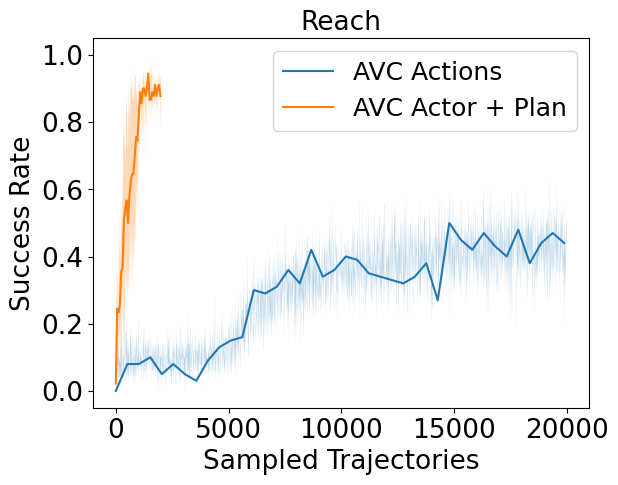
\includegraphics[width=\textwidth]{images/Plan_vs_Actions/Reach.png}
    \caption{Reach environment, One expert demonstration. Comparison of the action optimization mode (blue) and actor planner optimization mode (orange).
    Each experiment was repeated twice. The shaded region indicates the standard variation between runs. }
  \end{subfigure}

  \hfill

  \begin{subfigure}{0.48\textwidth}
    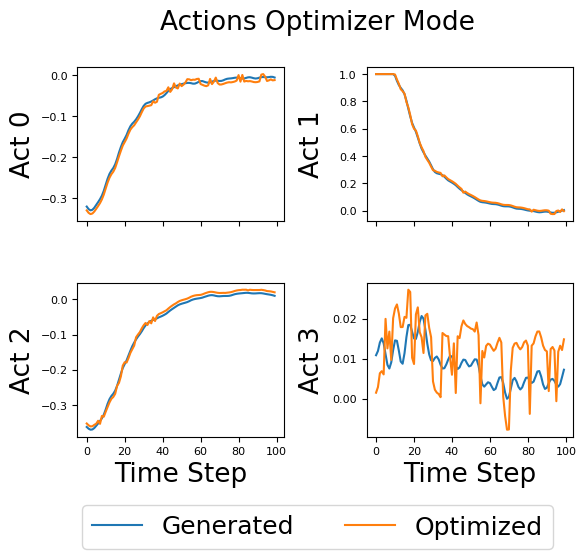
\includegraphics[width=\textwidth]{images/Plan_vs_Actions/vector_changes/Actions Optimizer Mode.png}
    \caption{Optimized trajectories (orange) and trajectories generated by the actor (green). 
    The experiments have four action dimensions, which are depicted in the 
    four plots per figure. 
    The gradient from the critic was applied to the actions.}
    \label{fig:direct_actions}
  \end{subfigure}
  \begin{subfigure}{0.48\textwidth}
    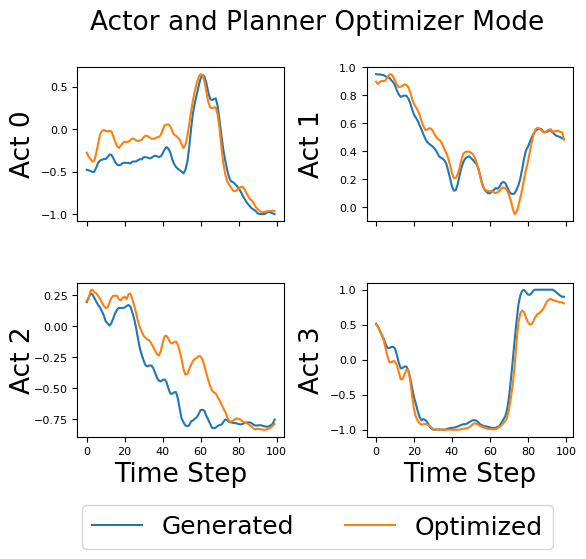
\includegraphics[width=\textwidth]{images/Plan_vs_Actions/vector_changes/Actor and Planner Optimizer Mode.png}
    \caption{Optimized trajectories (orange) and trajectories generated by the actor (blue). 
    The experiments have four action dimensions, which are depicted in the 
    four plots per figure. The gradient from the critic was applied to the actor and planner.}
    \label{fig:ac_pl_actions}
  \end{subfigure}
  \caption{Comparison of two optimization modes.}
  \label{fig:action_vs_actor}
\end{figure}

In Section \ref{sec:inf_time_search}, we discussed using different modes of optimization during inference time to optimize the action sequence. In this section, 
we showcase the difference between optimizing the action sequence directly and optimizing the actor and planner weights. We tested the two different 
modes in the reach environment given a single observation per trajectory. For the direct 
action optimization runs we used 20000 sampled episodes to see, if \ac{rl} took place at all, as for the first 2000 episodes no improvement above 
\ac{il} performance is seen. For this reason, we only repeated the experiment twice, as it took a long time to compute. The results are depicted in figure 
\ref{fig:action_vs_actor}. It is obvious, that the optimization mode is key to the \ac{rl} performance. 


In the bottom row of Figure \ref{fig:action_vs_actor}, the original generated trajectories (green) for the four action dimensions 
are shown alongside the optimized trajectories (orange) obtained using the gradient from the critic. We call the optimization mode 
where we apply the gradient directly to the actions "action optimization mode", and the optimization mode where we apply 
the gradient to the actor and planner networks and recalculate the trajectories given the changed networks "actor planner 
optimization mode".

We hypothesize that 
the actor planner optimization mode's much faster convergence rate is due to the actor and planner networks ability to 
encode an informed representation of the useful trajectory space. This informed representation guides the gradient search 
given by the critic, leading to more efficient exploration. Figure \ref{fig:direct_actions} illustrates the trajectory 
changes resulting from the action optimization mode, while Figure \ref{fig:ac_pl_actions} displays 
the trajectory changes resulting from the actor planner optimization mode.

We observe that the actor planner 
optimization mode produces a structured search, whereas the direct action optimization mode's trajectory changes are less structured.

Following the insights presented in this section, we will use the actor planner optimization mode for all experiments.



\subsection{Fine Tuning}
\label{sec:fine_tuning}

\begin{figure}[htbp]
  \centering
  \begin{subfigure}[t]{0.45\textwidth}
    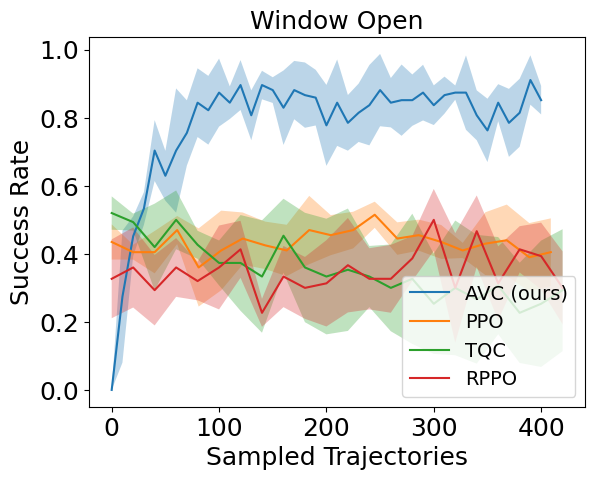
\includegraphics[width=\textwidth]{images/4_400/Window Open.png}
    \caption{Window Open environment, 4 expert demonstrations.}
  \end{subfigure}
  \begin{subfigure}[t]{0.45\textwidth}
    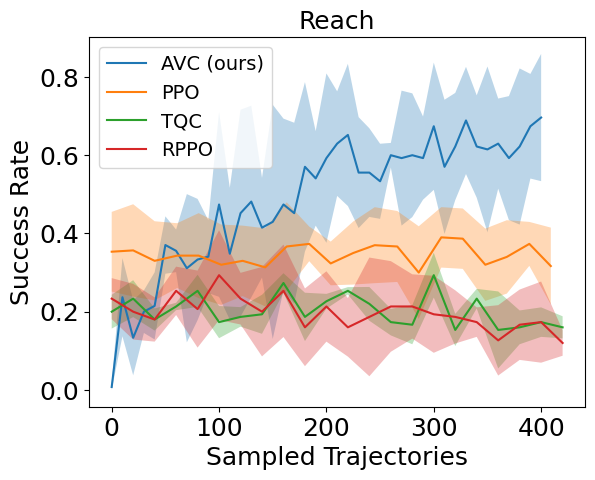
\includegraphics[width=\textwidth]{images/4_400/Reach.png}
    \caption{Reach environment, 4 expert demonstrations.}
  \end{subfigure}
  \medskip
  \begin{subfigure}[t]{0.45\textwidth}
    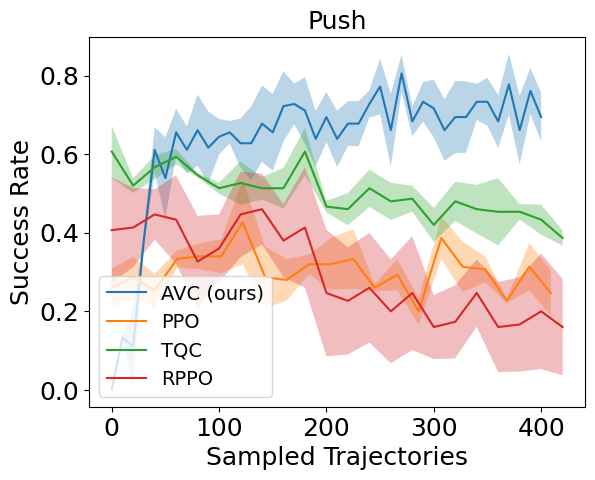
\includegraphics[width=\textwidth]{images/15_400/Push.png}
    \caption{Push environment, 15 expert demonstrations.}
  \end{subfigure}
  \begin{subfigure}[t]{0.45\textwidth}
    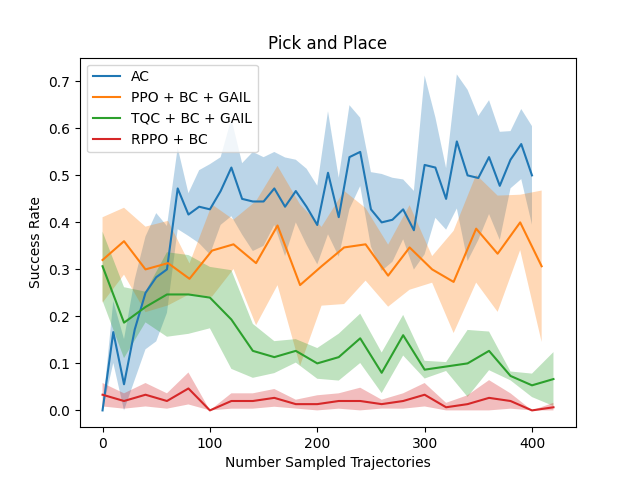
\includegraphics[width=\textwidth]{images/15_400/Pick and Place.png}
    \caption{Pick and Place environment, 15 expert demonstrations.}
  \end{subfigure}
  \caption{
    All baselines were pretrained using behavioral cloning with the given number of expert demonstrations. 
    The horizontal axis shows the number of sampled environment episodes, each with 100 steps. 
    One initial observation and, for \ac{rl}, a sparse reward signal at the end of each episode was provided. 
    The shaded area indicates the standard deviations from four runs per experiment.}
    \label{fig:finetuning}
\end{figure}

In this section, we analyze our algorithm in a fine-tuning setup. We provided the algorithms with 4 and 15 expert demonstrations per 
environment and used a relatively short \ac{rl} phase with 400 sampled trajectories consisting of 100 steps each. We 
repeated each experiment four times with 30 test trajectories per data point.

One problem we wanted to analyze that is typical in fine-tuning setups 
is "catastrophic forgetting" 
that can occur when the data distribution shifts. During the imitation phase, the learner only sees positive examples sampled according to 
the distribution induced by the expert, while the data distribution is induced by the learned policy in the \ac{rl} phase.
Our algorithm is more robust to this problem. We developed a lower bound on policy improvement including expert demonstrations in Section \ref{inference_time_planning}, which sets it 
apart from the policy improvement bound developed for \ac{trpo} \cite{TRPO}. \ac{trpo} assumes the whole dataset is sampled according to one policy, namely the policy of the last iteration. 
\ac{ppo} \cite{PPO}s relies on the same lower policy improvement bound using the same assumption, that is not fulfilled when you have a mixed dataset. 


We present our findings in Figure \ref{fig:finetuning}. 
For the environments Pick and Place and Push, we show the plots for 15 expert demonstrations. We found 4 expert demonstrations were not 
enough to meaningfully learn within 400 training episodes. The environments Reach and Window Open are easier to learn, so we display the 
experiments with 4 expert demonstrations each. In these environments, giving 15 expert demonstrations lead to near perfect performance from \ac{il} alone. 
All plots for all experiments can be found in Appendix \ref{chapter:additional_plots}.

We expected RPPO to be the least performant from our discussion of the curse of dimensionality in Section \ref{COD_AC}. As no current input 
is provided from the environment, RPPO has to keep track of all previous actions. \ac{ppo} and \ac{tqc} use positional encoding to indicate the current 
time step which makes the problem easier.

The algorithms guided by \ac{gail} did not improve meaningfully. We assume the limited amount of environment 
interaction was not proficient to learn a good discriminator to provide useful rewards for the reinforcement learners. 

During hyperparameter tuning we found, that the performance of the baselines was most 
reliant on the learning rate. High values lead to catastrophic forgetting. We chose the highest possible values before 
catastrophic forgetting took place. However, the performance from behavioral cloning, indicated by the first data point per plot, was mostly 
the best achievable performance. \ac{ppo} tends to do better than \ac{tqc} in the single observation setup in general, as expect due to the 
fact that \ac{tqc}'s strength as an off-policy algorithm lies in exploration. In our chosen setup, exploration is specifically hard, given no 
information from the environment during the trajectories.

We find that \ac{avc} is the only algorithm that can meaningfully improve its performance given the limited amount of environment interactions. 
We propose a contributing factor is that catastrophic forgetting is less pronounced in the \ac{avc} algorithm, as discussed earlier in this section and in Section \ref{inference_time_planning}, 
which makes it specifically suitable for fine-tuning.



\subsection{Guided/ Reinforcement Learning}
\label{sec:g_ref_ler}
In this section, we test the performance of \ac{avc} given minimal expert guidance on the Reach and Window Open environments.
With this setting, the algorithms must learn most of the behavior from \ac{rl}, but the expert
demonstration is needed to overcome the initial search problem. We only provide sparse reward and one observation per trajectory, thus finding the first viable solution by unguided
trial and error is unviable for most problems. However, we found the Drawer Close environment can be learned without any expert guidance.

We use \ac{ppo}, \ac{tqc} and RPPO for our baselines, as described in the introduction. We don't use \ac{gail} but make use of pretraining, as we focus on \ac{rl}. The results
are shown in Figure \ref{fig:guided_ref}.

\begin{figure}[htbp]
    \centering
    \begin{subfigure}[t]{0.32\textwidth}
      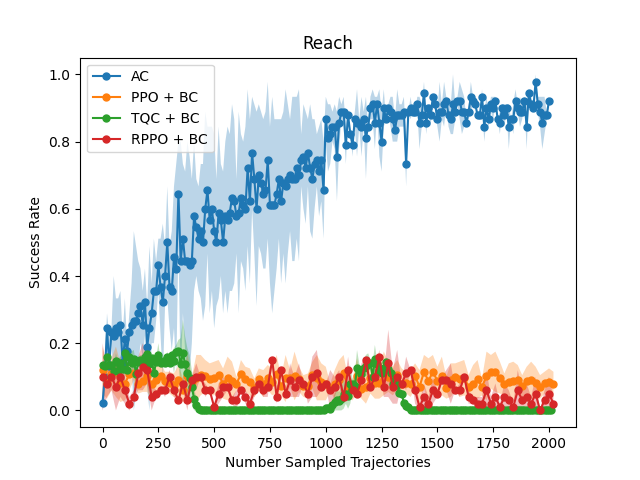
\includegraphics[width=\textwidth]{images/1_2000/Reach.png}
      \caption{One expert demonstration.}
    \end{subfigure}
    \begin{subfigure}[t]{0.32\textwidth}
      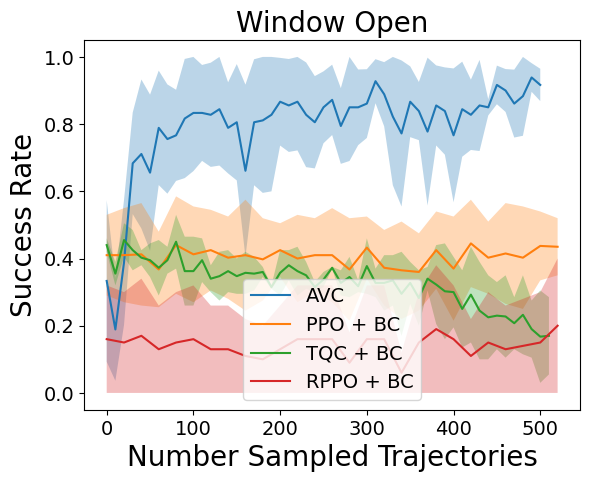
\includegraphics[width=\textwidth]{images/1_2000/Window Open.png}
      \caption{One expert demonstration.}
    \end{subfigure}
    \begin{subfigure}[t]{0.32\textwidth}
      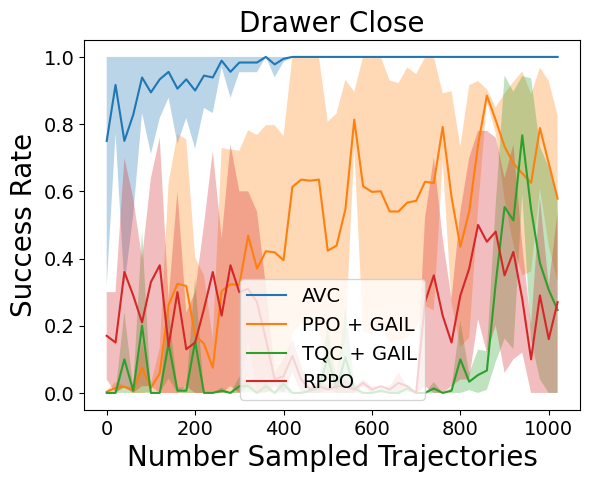
\includegraphics[width=\textwidth]{images/0/Drawer Close.png}
      \caption{Zero expert demonstrations.}
      \label{fig:drawerclose}
    \end{subfigure}
    \medskip
    \begin{subfigure}[t]{0.45\textwidth}
      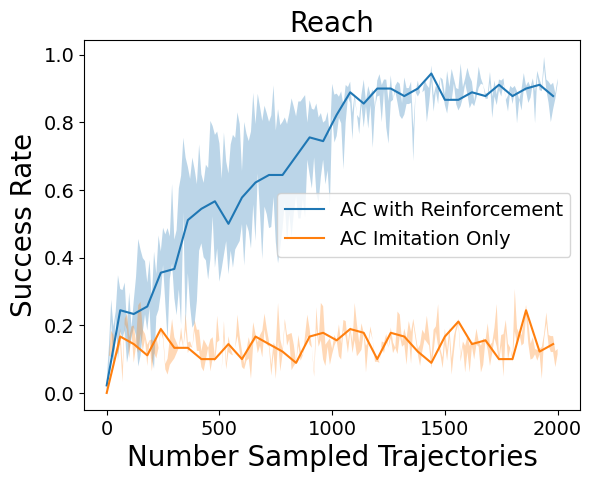
\includegraphics[width=\textwidth]{images/1_2000_imi/Reach.png}
      \caption{Reach environment. Comparison between pure \ac{il} and \ac{rl}.}
    \end{subfigure}
    \hfill
    \begin{subfigure}[t]{0.45\textwidth}
      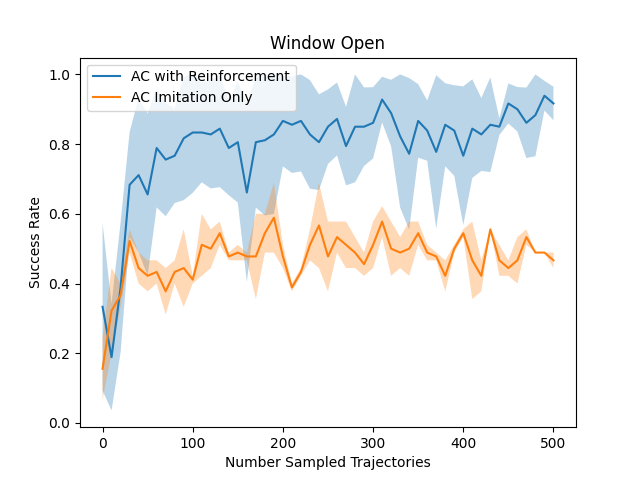
\includegraphics[width=\textwidth]{images/1_2000_imi/Window Open.png}
      \caption{Window Open environment. Comparison between pure \ac{il} and \ac{rl}.}
    \end{subfigure}
    \caption{
    All baselines were pretrained using behavioral cloning with the given number of expert demonstrations, where demonstrations were provided. 
    The x-axis shows the number of sampled environment episodes, each with 100 steps. On the bottom row, 
    the x-axis displays equal amount of compute for the pure \ac{il} experiment and the \ac{rl} experiment. 
    One initial observation and, for \ac{rl}, a sparse reward signal at the end of each episode was provided. 
    The shaded area indicates the standard deviations from three runs per experiment.}
    \label{fig:guided_ref}
\end{figure}

The \ac{avc} algorithm was able to solve all environments with high success rates after 1000 or 2000 sampled trajectories. In Reach and Window Open, the initial performance
of behavioral cloning was not improved in the reinforcement phase by any of the baselines. Similar to our discussion in Section \ref{sec:fine_tuning},
we had to choose small learning rates to prevent catastrophic forgetting. With higher learning rates, all baseline algorithms dropped to $0 \%$ success rate and did
not recover in initial tests. We find from the experiments that the challenging one observation sparse reward environment is difficult for
actor critic algorithms. In these setups, \ac{avc} shows a significant improvement over the baselines.

Following, we investigate aspects of the baselines to understand, how much of the performance improvement of \ac{avc} can be explained by the algorithm. 

\subsubsection{Expert Demonstrations}
First we wanted to rule out that the performance difference comes mainly from our behavioral cloning setup. As \ac{ppo} and \ac{tqc} natively don't make use of expert demonstrations,
we pretrained them using behavioral cloning. We expected that after pretraining, at least one successful trajectory would be sampled in the training phase, thus
helping to overcome the initial search problem. We find that all algorithms perform significantly above $0\%$ success rate, so we conclude that all algorithms had
sufficient guidance to find further successful trajectories. To further rule out that our methodology gives an unequal advantage to our algorithm, we tested all algorithms with 
zero expert demonstrations on the 
Drawer Close environment. We find, that random trajectories can already solve the environment with about $20\%$ success rate, so no expert guidance is needed to learn a feasible behavior.
The results are shown in Figure \ref{fig:drawerclose}.

Notable, \ac{avc} performs significantly better then the baselines at the first data point of the plot. This is unexpected, since it indicates 
random behavior from randomly initialization of the policies. In further tests, we found that the initial success rate is either close to one or close to zero for all policies depending 
on the initialization. 

This is likely due to the fact, that the initial observations for the Drawer Close environment are close in $L_2$ distance, thus a random policy will act similar in all environments. 
We find if a behavior solves one environment, there is a high probability that it will solve all environments. In the three runs of the experiment, \ac{avc} was randomly initialized to have a high success rate in two runs, while \ac{ppo} and \ac{tqc} had no 
initial success. We did not have time to repeat the experiment until the initial performance of the algorithms converge. However, in train mode, 
all algorithms sample trajectories randomly in the initial training phase. 

We set the initial random phase to 1000 steps or 10 trajectories, so all algorithms had access to some successful trajectories with high probability. While the initialization was an advantage 
for our algorithm in these experiment runs, it can still clearly be seen, that our algorithm is more stable with significantly smaller variance in its performance compared to the baselines. In a later 
section, we also conduct an experiment on the Drawer Close environment with continued observations, as seen in Figure \ref{fig:dense_ref}. We will discuss the figure in more detail later. It provides 
further evidence for the effectiveness of our approach in environments with no expert guidance. The overall high variance in the runs shown from the baselines can be explained by the sparse rewards, which provide highly non-linear feedback. 
\ac{avc} rapidly improved to perfect performance within about 400 steps.

\subsubsection{Neural Network Architecture}
Next, we wanted to rule out that the observed performance gain of \ac{avc} over the baselines comes mostly from increased performance in \ac{il} 
from the different underlying neural network architectures. \ac{avc} uses transformer encoders for the actor and 
critic, while the \ac{tqc} and \ac{ppo} implementations use MLPs and the RPPO implementation uses a GRU.

We tested the performance of \ac{avc} using pure \ac{il} shown on the bottom row of
Figure \ref{fig:guided_ref}. We find \ac{avc} has similar \ac{il} performance to behavioral cloning for our baselines with strong inductive bias. However, it significantly benefits from the reinforcement phase.

Overall, we take these finding as evidence for the effectiveness of the \ac{rl} aspect of the \ac{avc} algorithm.


\section{Reinforcement Learning from Sparse Rewards in Continued Observation Environments}
\label{sec_exp_con_obs}
In this section we test the relaxation of the \ac{avc} algorithm to \ac{mdp} environments, developed in Section \ref{sec:relax_dense}, with the environment state given as an observation after each step.
We use sparse rewards 
and compare \ac{coavc} to \ac{ppo} and \ac{tqc} on the Reach, Window Open and Drawer Close environments. Apart from 
providing an observation per time step,
we use the same setup as described in previous sections. The results are shown in Figure \ref{fig:dense_ref} for three runs per experiment.

\begin{figure}[htbp]
  \centering
  \begin{subfigure}[t]{0.45\textwidth}
    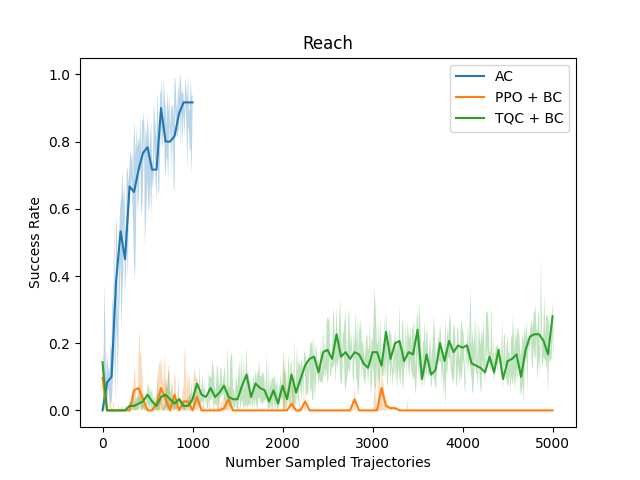
\includegraphics[width=\textwidth]{images/dense_1/Reach.png}
    \caption{One expert demonstration.}
  \end{subfigure}
  \hfill
  \begin{subfigure}[t]{0.45\textwidth}
    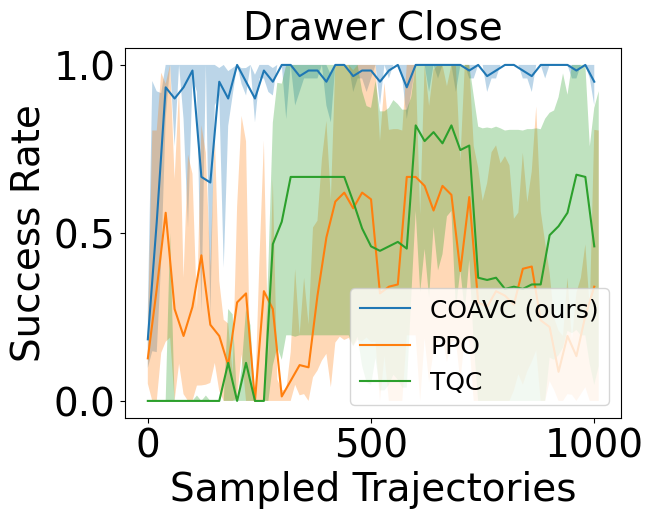
\includegraphics[width=\textwidth]{images/dense_0/Drawer Close.png}
    \caption{No expert demonstrations.}
  \end{subfigure}
  \medskip
  \begin{subfigure}[t]{0.45\textwidth}
    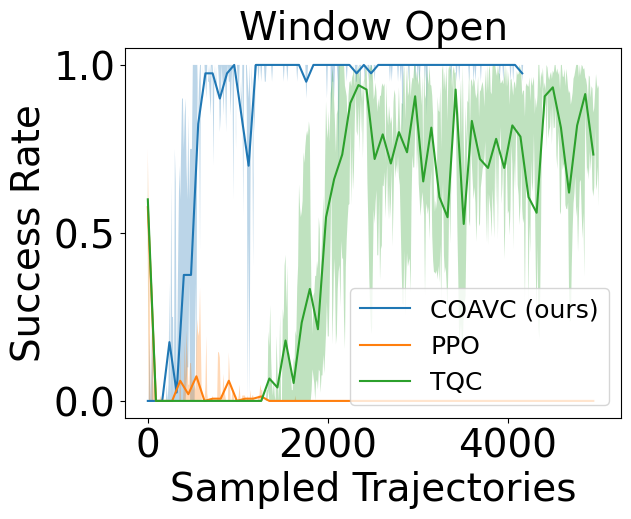
\includegraphics[width=\textwidth]{images/dense_1/Window Open.png}
    \caption{One expert demonstration.}
  \end{subfigure}
  \hfill
  \begin{subfigure}[t]{0.45\textwidth}
    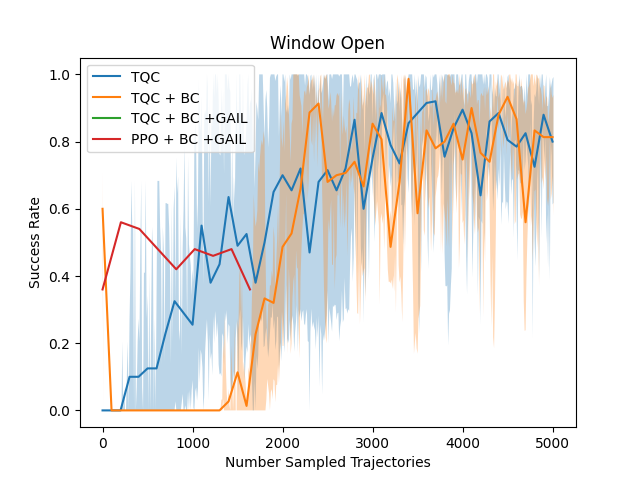
\includegraphics[width=\textwidth]{images/TQC_bc_GAIL_vs_ref/Window Open.png}
    \caption{Comparison between \ac{tqc} with no expert demonstrations and expert guided baselines.}
    \label{fig:TQC_0_vs_exp}
  \end{subfigure}
  \caption{All baselines were pretrained using behavioral cloning with the given number of expert demonstrations. 
    The x-axis shows the number of sampled environment episodes, each with 100 steps. 
    Continued observations and a sparse reward signal at the end of each episode was provided. 
    The shaded area indicates the standard deviations from three runs per experiment.}
    \label{fig:dense_ref}
\end{figure}

First, we note that both baseline algorithms exhibit similar performance in behavioral cloning as in the single 
observation setup. This is unsurprising as behavioral cloning does not rely on interactions with the environment.

After the first data point, both algorithms sharply drop to near zero success rate, which displays that catastrophic forgetting is more 
pronounced than in the single observation environment. We explain this with the distribution shift after training starts. A policy trained by \ac{il} 
will induce a different distribution of observations than the expert data. This breaks the \ac{iid} assumption for observations in addition to the changed distribution of rewards. 
In the single observation case for \ac{ppo} and \ac{tqc}, this assumption was not broken for the observations, 
since all observations are computed from the first observation. The distribution of the first observations is a constant of the environment.

PPO did not find solutions to the Reach and Window Open environments, 
but we find \ac{tqc} got about $20 \%$ success rate on Reach and achieved about $80 \%$ success rate on Window Open levelling out after about 2500 episodes. 
The superior performance of \ac{tqc} over \ac{ppo} is expected, as \ac{tqc} tends to perform better in environments where exploration is important. As \ac{tqc} now gets 
feedback from its actions on the environment, the better exploration is an advantage over PPO.

In particular, as \ac{tqc}'s performance drops to about $0 \%$ for the Window Open 
environment after the first data point, we wanted to analyze if \ac{tqc} uses the guidance from the expert at all, or if it starts from 
no usable knowledge about the environment. To do this, we also conducted the experiment three times with no initial behavioral cloning. The results are shown in 
Figure \ref{fig:TQC_0_vs_exp}. We observe that \ac{tqc} can solve the environment within 5000 steps from no expert demonstrations in one case, but does not find a good policy in the other two. 
We propose pretraining from behavioral cloning is a useful bias for the algorithm to find feasible solutions quicker with higher probability.

Following this insight, 
we also conducted the Window Open experiment in \ac{mdp} setting with \ac{gail} to make better use of the provided expert demonstration. We find our initial 
baseline with pretrained \ac{tqc} performs best. This is probably due to the fact, that \ac{gail} makes no use of the sparse reward. Additionally 
the authors mentioned in the paper \cite{ho2016generative}, that \ac{gail} is not more efficient in terms of environment interactions then \ac{trpo} with rewards. A large number of 
environment interactions are needed, before the discriminator of \ac{gail} provides useful rewards for the learner. We suppose that is a reason, why \ac{gail} does not perform 
well in our setting, where a relatively small amount of environment interactions are used.

We also included results for the Drawer Close environment with no expert demonstrations. All algorithms perform better than in the single observation environment, 
but \ac{coavc} is the only algorithm with stable performance. It found a solution with near perfect success rate in all three runs quickly.

Overall, \ac{coavc} performs well in all shown environments. Especially in the Reach environment it is the only algorithm that finds a feasible solution while it 
converges much quicker and has a more robust behavior in general. 






\subsection{Comparison of Continued and Single Observation}
\label{sec:com_coavc_avc}
In this section, we compare \ac{coavc} and AVC to investigate if \ac{coavc} makes use of the additionally provided information from the continued observations. 
The results are shown in Figure \ref{fig:dense_vs_single}.

\begin{figure}[htbp]
  \centering
  \begin{subfigure}[t]{0.32\textwidth}
    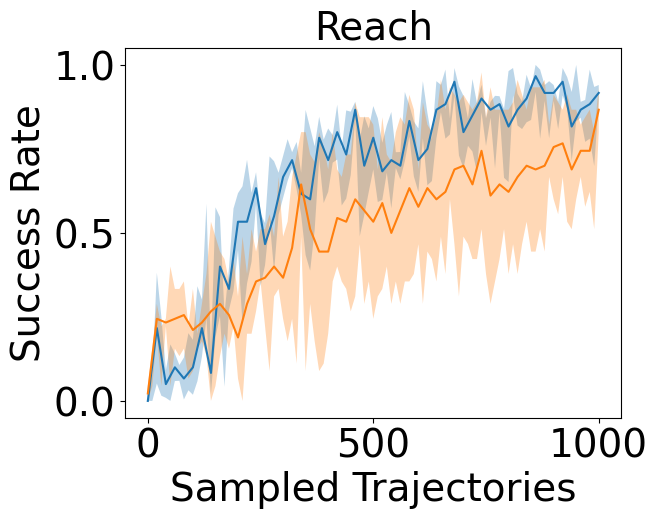
\includegraphics[width=\textwidth]{images/dense_vs_sparse_1/Reach.png}
    \caption{One expert demonstration.}
  \end{subfigure}
  \hfill
  \begin{subfigure}[t]{0.32\textwidth}
    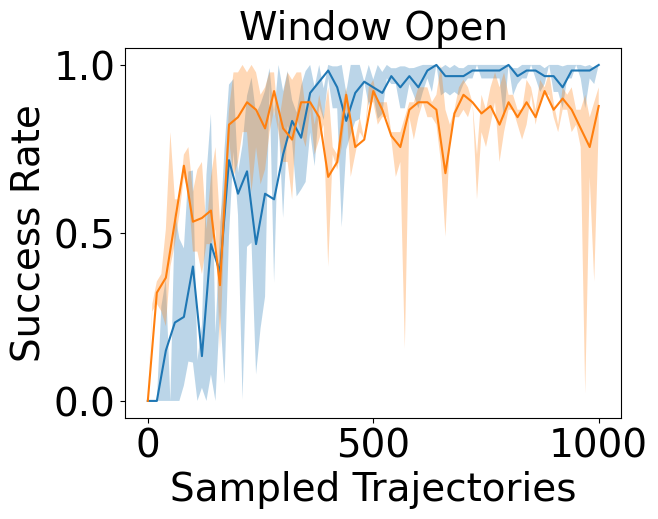
\includegraphics[width=\textwidth]{images/dense_vs_sparse_1/Window Open.png}
    \caption{One expert demonstration.}
  \end{subfigure}
  \hfill
  \begin{subfigure}[t]{0.32\textwidth}
    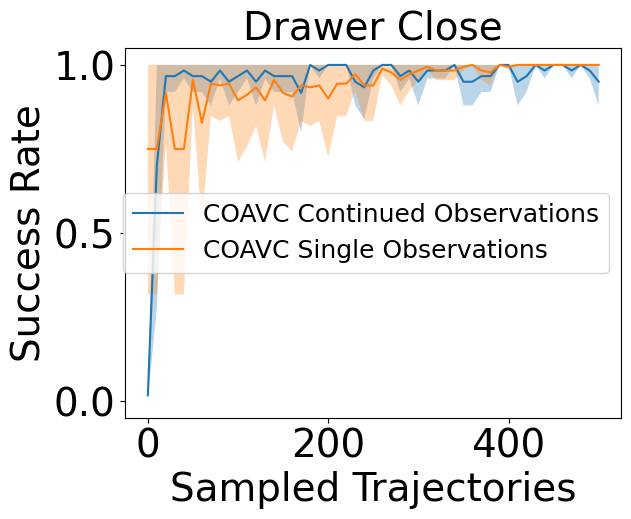
\includegraphics[width=\textwidth]{images/dense_vs_sparse_0/Drawer Close.png}
    \caption{Zero expert demonstrations.}
  \end{subfigure}
  \caption{Comparison of \ac{avc} in single observation and \ac{coavc} in continued observation \ac{mdp} environments. Each experiment was repeated three times with 30 evaluation episodes per data point.
  }
  \label{fig:dense_vs_single}
\end{figure}

We observe that in Reach and Drawer Close, \ac{coavc} converges quicker. Especially in Reach, we see a stable improvement from \ac{coavc} over AC. In Drawer Close, the difference is 
small, which is mainly due to the fact that \ac{avc} already solves the environment very quickly. Note however, that \ac{coavc} had worse initial performance then \ac{avc} in the shown experiments. 
As previously discussed, the initial performance is determined by random initialization of the networks and can exhibit substantial 
variance.

The observation that \ac{coavc} achieved convergence at a faster rate than AVC, despite starting with inferior initializations in 
all three runs, provides additional support for the proposition that \ac{coavc} makes effective use of the continued observations.

In the Window Open environment, \ac{coavc} initially converged slower but 
reached near perfect performance quicker then AC. We suppose this is due to the different optimization modes used for the two algorithms. Recall, that \ac{avc} optimizes the whole 
trajectory at the beginning, while \ac{coavc} makes small improvements per time step due to self-imposed inference time constraints. During inference time, the critic of 
\ac{avc} can make larger changes to the trajectory proposed by the actor. In other words, \ac{coavc} makes smaller moves towards the critic target than AC. Also, out of time constraints, we could 
not conduct a hyperparameter search for \ac{coavc}. It is possible, that \ac{coavc} would converge quicker, given more optimization steps per inference step or a higher inference optimization 
learning rate $\alpha_{\mathrm{inf}}$.

AVCs performance is close to \ac{coavc}. We propose this is due to the fact, that \ac{avc} uses the information about the environment 
from the expert demonstrations effectively to search for new candidate solutions. As discussed in Section \ref{ref:com_opt_modes}, \ac{avc} searches on a prestructured subspace given the "knowledge" of the 
actor. This means it does not conduct random search even though it does not get any feedback from the environment. This is probably a key for the good performance of \ac{avc} and \ac{coavc} and explains 
the relative close performance of both algorithms. Overall, we find that \ac{coavc} works well in the tested environments and outperforms all baselines in the \ac{mdp} setting with sparse rewards.